\documentclass{article}
% \setlength{\parskip}{1em}
\title{Political Information in Bureaucratic Policymaking}
\author{Devin Judge-Lord} % \\ JudgeLord@Wisc.edu}


\date{\today} 
 %\setlength{\parskip}{1em}
% \usepackage[round, sort, comma]{natbib}
% \setcitestyle{notesep={, },round,aysep={},yysep={,}}

%\setlength{\parindent}{0pt}

% \usepackage[authordate,strict,backend=bibtex8,babel=other, doi=false, url=false, isbn=false, uniquename=false, maxcitenames = 2, uniquelist=false,%
% bibencoding=inputenc, natbib]{biblatex-chicago}
%\usepackage[authordate, backend=biber, doi=false, url=false, isbn=false, uniquename=false, maxcitenames = 2, uniquelist=false, natbib]{biblatex-chicago}



% ---------------------------------------
%   REFERENCES
% ---------------------------------------
\usepackage{natbib} %[round, sort, comma]{natbib}
  \bibpunct[: ]{(}{)}{;}{a}{}{,}
%\usepackage[nottoc,numbib]{tocbibind} % numbers bib. in table of contents


% ---------------------------------------
%   MARGINS AND SPACING
% ---------------------------------------
\usepackage[margin=1in]{geometry} 
\usepackage{setspace} % line spacing


% ---------------------------------------
%   TABLES AND FIGURES
% ---------------------------------------
\usepackage{graphicx} % input graphics
\graphicspath{ {./Figs/} }

\usepackage{float} % float parameters
\usepackage{placeins} % \FloatBarrier: prevent floats spilling across sections
\usepackage{subcaption} % subfloats with individual captions
\usepackage{multirow} % multicolumn and multirow
\usepackage{booktabs} %? for toprule, midrule etc
\usepackage{dcolumn} % decimal-aligned columns

\usepackage{tikz}
\usetikzlibrary{positioning}
\usetikzlibrary{shapes.geometric}
\usetikzlibrary[patterns]

% ---------------------------------------
%   MATH
% ---------------------------------------
\usepackage{amsmath}
%  Math symbols (depends on whether you customize typeface)
%  \usepackage{amsfonts}
%  \usepackage{mathrsfs}
\usepackage{amssymb}
  %  \newcommand{\E}{\mathrm{E}}
  %  \newcommand{\Var}{\mathrm{Var}}
  %  \newcommand{\Cov}{\mathrm{Cov}}
  %  \newcommand{\plim}{\mathrm{plim}}
  %  \renewcommand{\L}{\mathcal{L}}
  %  \renewcommand{\d}{\mathrm{d}}
  %  \newcommand{\R}{\mathbb{R}}


% ---------------------------------------
%   TYPEFACE AND TEXT STYLES
% ---------------------------------------


% \usepackage{fontenc} 
% advisable to include for nitty-gritty details
% (ligatures, kerning & other typographical things)

% \usepackage[usenames, dvipsnames]{xcolor} % extra colors
\usepackage{hyperref} % hyperlinks
   \hypersetup{
     colorlinks = true, 
     citecolor = black, 
     linkcolor = blue,
     urlcolor = blue}

\usepackage{comment} % provides {comment} environment
\usepackage{enumitem} % allows [nosep] option for lists

\usepackage{endnotes}

\makeatletter
\renewcommand\@makeenmark{%
  \textsuperscript{\normalfont\textcolor{blue}{\@theenmark}}%
}
\newcommand{\uncolormarkers}{%
  \renewcommand\@makeenmark{%
    \textsuperscript{\normalfont\@theenmark}%
  }%
}
\makeatother


\newcommand{\exclude}[1]{\StopSearching ##1\StartSearching}

\usepackage{ragged2e}


% FOR DAVE: %%%%%%%%%%%%%%%%%%%%%%%%%%%
% \let\footnote=\endnote
% \renewcommand{\footnotesize}{\normal}
%%%%%%%%%%%%%%%%%%%%%%%%%%%%%%%%%%%%%%%
\begin{document}
% FOR DAVE: %%%%%%%%%%%%%%%%%%%%%%%%%%
% \large
% \doublespace
% \RaggedRight
%%%%%%%%%%%%%%%%%%%%%%%%%%%%%%%%%%%%%%

\maketitle
% \tableofcontents
% \abstract{This dissertation is about public pressure campaigns that target U.S. federal agency rulemaking, a technocratic policy process in which participation is usually limited to a few policy insiders. Occasionally, however, public pressure campaigns help make agency rules some of the most hotly contested policies of our time. I examine who organizes public pressure campaigns and why, whether these campaigns affect congressional oversight, and whether they affect policy. Answering these questions informs our understanding of bureaucratic politics as well as interest group lobbying, organizing, and mobilizing tactics. Most comments that federal agencies receive on their draft policies come from ordinary people who were inspired by a public pressure campaign. Yet leading theories of bureaucratic policymaking neither explain nor account for these occasional bursts of civic engagement. This dissertation develops and tests theories about the roles of individuals, organizations, coalitions, and social movements in bureaucratic policymaking. I argue that pressure campaigns build movements, attract policymakers' attention, and systematically counter corporate power by generating political information---information about public demands.   I make four main contributions:
  
  First, drawing on scholarship on social movements, interest group behavior, and lobbying, I identify three reasons for lobbying organizations to mobilize ordinary people. Each logic suggests a different observable pattern of public engagement, and I analyze millions of public comments on thousands of agency rules to develop the first systematic measures of public engagement in bureaucratic policymaking. Contrary to other forms of lobbying, I find that mass comment campaigns are almost always a conflict expansion tactic rather than well-resourced groups creating an impression of public support. Most public comments are mobilized by public interest organizations, not by narrow private interests or astroturf campaigns. However, the resources and capacities required to launch a campaign cause a few larger policy advocacy organizations to dominate.
  
  Second, building on theories of political oversight, I theorize that mass engagement in bureaucratic policymaking may alert elected officials to political opportunities and risks, thus affecting oversight behavior. I assess this argument by analyzing correspondence between members of Congress and agency officials on proposed rules with and without mass engagement. I find that public pressure campaigns are correlated with congressional attention and that coalitions with more congressional support are more likely to achieve their policy goals.
  
  Third, I integrate intuitions about outside lobbying and oversight into a broader theory of how public pressure campaigns may affect policy by producing potentially influential political information. I suggest four causal mechanisms by which lobbying may influence bureaucrats and expand leading formal models of interest group influence in bureaucratic policymaking to account for political information. I then test these models using a mix of hand-coding and computational text analysis methods.   
  
  Fourth, I advance the literature on social movement pressure through a case study of the environmental justice movement. I show that pressure campaigns are more than a lobbying tactic; they are also an institutionalized form of contentious politics over the distribution of governmental power. I examine the discursive effects of environmental justice claims both qualitatively and quantitatively, including the role of Native activists and environmental groups in shaping federal policy. I find that agencies frequently ignore environmental justice concerns but are more likely to add language addressing environmental justice in their final rules when public comments raise environmental justice concerns. I conclude with implications for theories of bureaucratic policymaking and future research, a review of dominant ways of thinking about public comment periods, and proposed reforms for public participation in policymaking.}
% 
\includegraphics[height = .5cm]{spam}
% \newpage

The broader project aims to better understand the role of ordinary people in bureaucratic policymaking. 
I develop theories of why mass engagement occurs and how it may affect policy. To assess these theories, I tackle three related empirical questions: (1) Why does it occur?; (2) How does it affect the oversight behaviors of agencies' political principals?; and %These questions drive two initial empirical chapters.
(3)  Does mass engagement in bureaucratic policymaking affect policy?
% I then use my new measures of the political information that lobbying coalitions create by going public to test whether mass engagement explains variation in agency rulemaking and rules.% But first, I must develop a measure of ``going public.'' % and why it occurs.

\paragraph{Part 1. Why do agencies (occasionally) get so much mail?} %: Lobbying coalitions, mass comments, and political information in bureaucratic policymaking
% Scholars of bureaucratic policymaking have focused on the sophisticated lobbying efforts of powerful interest groups. Yet agencies occasionally receive thousands or even millions of comments from ordinary people. Why? Why do individuals comment when they seemingly have no new information to offer and no power to influence decisions? Who inspires them and to what end? How, if at all, should scholars incorporate mass commenting into models of bureaucratic policymaking? I argue that mass commenting produces political information about the coalition that mobilized it. 
% QUESTION 1\textbf{Puzzle:} 
Why do some rules receive many comments from ordinary people and some do not?
% Why do people comment on draft policies when they seem to have no new information to offer and no power to influence decisions? Who inspires them and to what end? 
% THEORY AND METHODS 1
% Answering this question requires a theory explaining variation in mass engagement. 
The literature suggests two possible explanations for variation in mass engagement; groups may leverage public support as a lobbying resources (``grass roots'' mobilization) or groups with more resources may leverage those resources into impression of public support (sometimes called ``astro-turf'').
%Using new measures of public engagement in agency rulemaking, I identify the conditions under which it occurs and produces different politically-relevant information. 
% The dependent variable is the number of people engaged.
I theorize that public support explains variation in mass engagement. That is, unlike other forms of lobbying, it not primarily driven by groups with more resources. Specifically, I anticipate three patterns:
(1) When a coalition is disadvantaged in insider politics but as more public support than opposing coalitions, they are more likely to ``go public'' to bolster their lobbying effort (assuming they have the resources to do so). More public support yields more engagement, more effort per participant, and contagion beyond those mobilized directly. (2) Coalitions with less support may ``counter-mobilize'' with proportionally smaller results. That is, groups with more resources but less public support only mobilize when their opponents do so. (3) Finally, coalitions may mobilize for reasons unrelated to the policy at hand, yielding significant mass engagement but without a corresponding insider lobbying effort. 
Because the vast majority of comments are inspired by interest-group campaigns, finding their cause requires a method to link comments to the lobbying coalitions that mobilized them.  
To link individual comments to the more sophisticated lobbying efforts they support, I use text reuse and clustering methods to capture formal and informal coalitions.
Measures of mass engagement include 
%(1) total public comments, % $\sim$ zero-inflated negative binomial; 
(1) comments per coalition, % $\sim$ negative binomial; 
(2) effort per comment, % $\sim$ truncated normal; 
(3) share of comments per coalition mobilized indirectly (i.e. the potential for conflict spread).
With measures, I test whether variation in engagement explains variation in oversight behavior (part 2) and policy outcomes (part 3).
% (4) type of campaign. % $\sim$ multinomial. 
%Model 1 is one observation per rule. Models 2-4 are one observation per coalition per rule. Explanatory variables include agency alignment with Congress and the president (models 1-4), coalition alignment and unity (models 2-4), whether a coalition is driven more by public or private interests (models 2-3).%, part of the DV in model 4).

%\paragraph{Step 2. Are elected officials more or less likely to engage after mass public engagement?} 
\paragraph{Part 2. Does mass engagement affect political oversight?} The political information signaled by mass engagement may serve as a ``fire alarm,'' altering principals to oversight opportunities or ``warning signs'' altering them to political risks.
When a coalition mobilizes successfully, %especially if it generates a perceived consensus in expressed public sentiments, 
elected officials ought to be more likely to engage on their behalf and less likely to engage against them.
% This suggests an addendum to Hall and Miler's (2008) finding that members are more likely to engage in rulemaking when they have been lobbied by a like-minded interest group.
% When interest groups lobby elected officials to engage in rulemaking, they may be more likely to engage when aligned with most commenters than when opposed.
% If politicians learn from political information, they will be even more likely to engage when lobbied by a coalition that includes a public interest group's with a large mass-comment campaign, and less likely when lobbied by a coalition dominated by private interests opposed by a mass comment campaign. 
% MEASUREMENT  2
To assess these hypotheses, I count the number of times Members of Congress engage the agency before, during, and after comment periods on rules where lobbying organizations did and did not go public. I then use text analysis to compare legislators' sentiments and rhetoric to that used by each coalition.
% Similarly, I asses the involvement of presidential appointees and the President's Office of Management and Budget before and after public comment, again comparing rules that were and were not targeted by a campaign (a difference-in-difference). 
% As a validity check, I also look for remarks by elected officials and judges on the level of public engagement.
Dependent variables include 
(1) the number of comments from Members of Congress on the rule %(total, those mentioning mass comments, and those mentioning organizations in the coalition), %All  $\sim$ zero-inflated negative binomial. 
(2) the share of supportive congressional comments, %  $\sim$  beta. 
(3) the similarity of words in comments from the coalition and Members of Congress. 

\paragraph{Part 3. Does mass engagement affect rulemaking and rules?} 
I theorize that the effects of political information on policy depend on the extent to which the strategic environment allows change and how political information is processed, both directly within agencies and indirectly through other actors (e.g. Members of Congress) whose appraisals matter to bureaucrats.
The main dependent variable is change in the rule text.
%Different inputs may yield different results: 
I systematically identify changes between draft and final rules, parse these differences to identify meaningful policy changes, and compare them to demands raised in comments to measure which coalition got their desired outcomes.% However, assessing policy change is difficult. Thus, I also use other measures of agency responses to lobbying efforts. 

% Chapter 1 Intro
% 
Paticipatory processes like public comment periods, where government agencies must solicit public input on draft policies, are said to provide political oversight opportunities \citep{Balla1998, Mccubbins1984}, democratic legitimacy \citep{Croley2003, Rosenbloom2003}, and new technical information \citep{Yackee2006JPART, Nelson2012}. %\footnote{These various goals are evident in the Proposed Recommendation on Public Engagement in Rulemaking from the Administrative Conference of the United States, which asserts that ``The opportunity for public engagement is vital to the rulemaking process, permitting agencies to obtain more comprehensive information, enhance the legitimacy and accountability of their decisions, and enhance public support for their rules'' \citep{ACUS2018}.}
%Public comment periods are purported to simultaneously produce technical information, accountability to elected officials, and responsiveness to public demands.
While recent scholarship on agency policymaking has shed light on the sophisticated lobbying by businesses and political insiders, we know surprisingly little about the vast majority of public comments which are submitted by ordinary people as part of public pressure campaigns.\footnote{As I show elsewhere \citep{Judge-Lord2019}, most comments submitted to regulations.gov are form comments, more akin to petition signatures than sophisticated lobbying. Indeed, aproximately 40 million out of 50 million (80\%) of these public comments mobilized by just 100 advocacy organizations.}
Activists frequently target agency policymaking with letter-writing campaigns, petitions, protests, and mobilizing people to attend hearings, all classic examples of ``civic engagement'' \citep{Verba1987}. Yet civic engagement remains poorly understood in the context of bureaucratic policymaking.

These occasional bursts of civic engagement in bureaucratic policymaking raise practical and theoretical questions for the practice of democracy.\footnote{In 2018, the Administrative Conference of the United States (ACUS) identified mass commenting as a top issue in administrative law. In their report to ACUS, \citet{SantAmbrogio2018} conclude, ``The `mass comments' occasionally submitted in great volume in highly salient rulemakings are one of the more vexing challenges facing agencies in recent years. Mass comments are typically the result of orchestrated campaigns by advocacy groups to persuade members or other like-minded individuals to express support for or opposition to an agency's proposed rule.'' 
Mass comment campaigns are known to drive significant participation of ordinary people in Environmental Protection Agency rulemaking \citep{Judge-Lord2019, Potter2017, Balla2018}. \citet{Cuellar2005}, who examines public input on three rules, finds that ordinary people made up the majority of commenters demonstrating ``demand among the mass public for a seat at the table in the regulatory process.'' } 
%To date, administrative law scholars have focused on practical and normative questions, much of this analysis depends 
These questions, in turn, hinge on unanswered empirical questions: Do these campaigns affect policy? If so, by what mechanisms? Existing research finds that commenters believe their comments matter \citep{Yackee2015JPART} and that the number of public comments varies across agencies and policy processes \citep{Judge-Lord2019, Libgober2018, Moore2017},
% and policy change is related to the number of comments in sample of nine rules \citep{Shapiro2008}, 
but the relationship between the scale of public engagment and policy change remains untested. 

To address this gap, I assess the relationship between the number of public comments and the amount of change between draft and final policy texts. Next, I assess the relationship between the number of people mobilized by each campaign and whether the campaign acheivied its policy goals. Finally, I theorize and test four mechanisms by which public input may affect bureaucratic policymaking. Each mechanism involves a distinct type of information that pressure campaigns may relay to policymakers: technical information, information about the likelihood of political consequences, information about the preferences of elected officials, or information about the preferences of the attentive public. Because scholarship on bureaucratic policymaking has focused on the power of technical information, where insider lobbying is most likely to matter and where outside strategies are least likely to matter, political scientists have largely overlooked mass mobilization as a tactic.

% To assess the relationship between mass engagement and policy change, I introduce a large new dataset of millions of public comments on agency rules and assess mass comment campaigns' impact on rulemaking processes and outcomes. % To assess the relationship between mass public participation and rule change, I outline four potential mechanisms by which public input may influence bureaucratic decisions. 
I find evidence consistent with the observable implications of mass comment campaigns influencing policymaking through [non-null results] but no evidence that mass engagement affects rulemaking processes or outcomes through [null results].




% Chapter 2 Methods
% In this section, I develop methods to attribute mass comments to the campaigns that mobilized them and measure the intensity of preferences expressed. 
To link individual comments to the more sophisticated lobbying efforts they support, I use text reuse and topic models to identify clusters of similar comments, reflecting formal and informal coalitions. Comments with identical text indicate which groups and coalitions also chose to run a mass comment campaign. Within each campaign, I measure the intensity and potential for the movement to grow. To measure intensity, I examine the ratio of high-effort and low-effort comments. To measure potential to grow, I measure the number of comments mobilized indirectly by the campaign.
The result is several new measures that paint a picture of mass commenting. Using these new measures of public engagement in agency rulemaking, I identify the conditions under which it occurs and produces different politically-relevant information. 

\subsubsection{Who lobbies?}
Previous studies of rulemaking stress the importance of coalitions \citep{Yackee2006a}. Scholars have measured coalitions of organized groups but have yet to be able to attribute citizen comments to the coalition that mobilized them.
% Metadata on participants in rulemaking including the date and author of comments (often including the type of author, i.e. business, business group, citizen, public interest group, etc.)% and briefs
% allows me to track and compare relative alignment across venues and over time to assess whose ideas and interests are reflected at each stage of policymaking and in policy processes over time. % and review, for example from a statute or executive order, to the agency rule(s), to review by the White House, to court opinions. 
Unfortunately, metadata on the authors of comments are often inconsistent and incomplete. As this information is key to identifying influential actors, improving these data is a significant data-organization task. I have collected a corpus of over 70 million comments on over 300,000 proposed rules. The first task will be linking these comments to other data on the rules. 

Text search matching organization and individual names across texts, especially those named as comment authors will help systematically link individuals to the groups that mobilized them.% who may participate in different coalitions and under different names over time. 
This helps to identify formal coalitions of organizations that sign onto the same comment as well as experts and citizens mobilized by advocacy campaigns to submit separate comments.

Having identified who is participating in rulemaking, the next step is to identify who is lobbying together.

\subsubsection{Who lobbies together?}
% political information example 
The Oceana coalition framed its mass mobilization effort to curb the  Bureau of Ocean Energy Management's 2017 Proposed Offshore Oil and Gas Leasing Program as a ``petition signed by 67,275 self-proclaimed United States residents,'' suggesting that organizations consider these efforts as akin to petitions. In the same statement, Oceana also claimed the support of ``more than 110 East Coast municipalities, 100 Members of Congress, 750 state and local elected officials, and 1,100 business interests, all of whom oppose offshore drilling,'' suggesting that claims of public and elected official support aim to provide similar kinds of political information. 

% lobbying together - cosigning 
When actors sign onto the same comment, it is clear that they are lobbying together. This generally takes two forms. Businesses and groups representing allied industries often co-sign carefully crafted suggestions that reflect their common interest. We expect this to occur when the benefits of coordination outweigh the costs \citep{Yackee2006JOP}. The other form this take is public campaigns that ask citizens to submit a form letter, often alongside other actions such as protests. These occasional bursts of civic participation may affect rulemaking \citep{Coglianese2001}, but this is yet to be tested. In the first form, many of the businesses are repeat players and I record them individually. In the second form, the advocacy groups are repeat players, and I recorded their participation, but it would be citizens who participate are likely not and I record the number of these comments as an amplitude parameter for the text they signed and I attribute form-letter texts to the advocacy groups promoting them.

Various businesses, advocacy groups, and citizens often comment separately even when they aligned. The comment process is open to anyone and it is often not worthwhile for all actors to coordinate their messages. There may be many dimensions of demands and it is unclear to which coalition many comments belong.

% Identifying when commenters change coalitions is key for testing policy feedback theories about how policies reorganize political coalitions. I do this by indexing rules over time and adding a parameter for the probability that an actor switches from one coalition to another at each point in time. This allows the model to achieve a better fit by reclassifying an actor after some point in time. These actor-specific and coalition-specific points in time are a key output of this approach required to test theories of how policies reorganize political coalitions. 

% Bounding the scope of this model (i.e. the policy system) is a challenge. On the one hand, each agency deals with many issues of interest to different coalitions. On the other hand, many lobby across multiple agencies. I opt to model coalition advocacy at a fine scale based on Office of Management and Budget agency sub-function codes, but I may try to link across related issues and agencies. 

In addition to mapping text re-use, I adapt several statistical models (Bayesian classifiers) of text to classify comments into coalitions. Classifying comments into common groups is a task well suited for a single membership topic model.\footnote{
This is in contrast to the mixture model I use to estimate the distribution of multiple topics in each document and each coalition in section \ref{principals-methods}
}. 
This model clusters documents by the frequency with which they use different words. Being classified together does not mean that the documents all address exactly the same distribution of substantive issues, just that how issues are discussed is similar relative to the full set of documents.
I start by modeling all comments on each rule (collapsing exactly identical comments to one document) with three topics, which I will then inspect to see how well the comments of named organizations were classified. If three topics appear to sensibly describe the conflict, I tag these topics as ``pro, con, other.'' 





In terms of the causal process theorized above, this section focuses on measuring and explaining organizations' lobbying choices (i.e. to only provide technical information or to also mobilize) and public response to mobilization campaigns (the frequency and effort with which people engage). The key explanatory variable is public support for the campaign. The bold arrows in figure \ref{fig:causal-whymail-test} indicate the relationships of interest for this step.

\begin{figure}[h!]
    \centering
    \caption{Step 1: Explaining Mass Mobilization and Mass Engagement} 
    \label{fig:causal-whymail-test}
\tiny
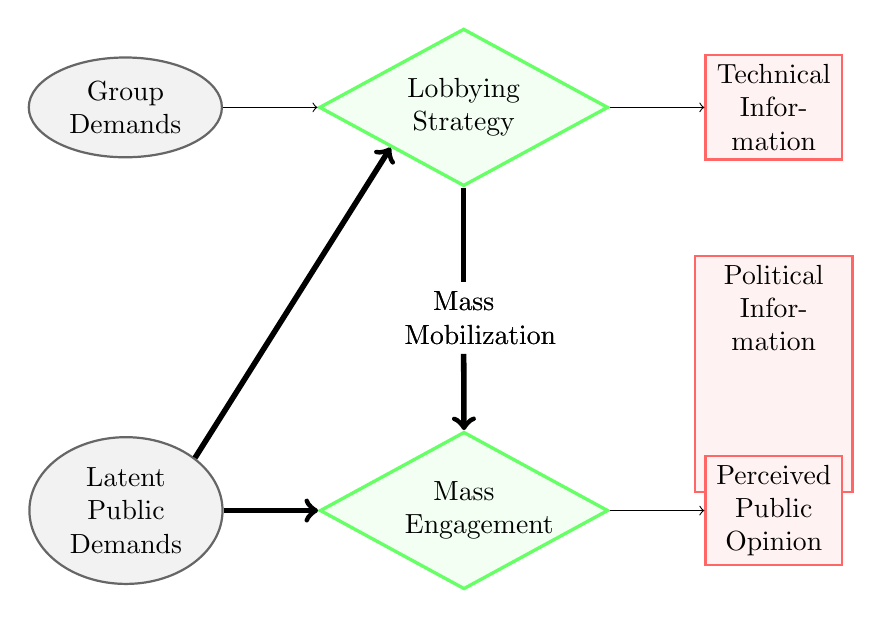
\begin{tikzpicture}[%
    node distance=1.2cm,
    auto,
    text width=1.5cm,
dnode/.style={diamond, align=center, aspect=2, fill=green!5,draw=green!60, very thick, minimum size=2cm},
squarednode/.style={rectangle, align=center, aspect=1, draw=red!60, fill=red!5, thick, minimum size=1cm},
pnode/.style={ellipse, align=center, aspect=1, draw=black!60, fill=black!5, thick, minimum size=1cm},
title/.style={rectangle, align=center, aspect=1, minimum size=2cm},
]

% Group Nodes
\node[pnode]      (groupdemands) {Group Demands};
\node[dnode]        (groupdecides) [right=of groupdemands] {Lobbying Strategy};
\node[squarednode]      (groupinfo) [right=of groupdecides] {Technical Information};


% Group Lines
\draw[->] (groupdemands.east) -- (groupdecides.west);
\draw[->] (groupdecides.east) -- (groupinfo.west);

% Titles
% \node[title]      (1) [above=of draft] {Policy};
% \node[title]      (2) [above=of groupdemands] {Preferences};
% \node[title]      (4) [above=of groupinfo] {Information/ Signal};
% \node[title]      (3) [above=of groupdecides] {Observed Behavior};
% \node[title]      (5) [above=of policy] {Policy'};

\node[text centered]      (mobilizing) [below=of groupdecides] {Mass\\ Mobilization};

% political info
\node[rectangle, minimum width =2cm, minimum height = 3cm, draw=red!60, fill=red!5,  thick]      (politicalinfo) [below=of groupinfo] {};

\node[text centered]      (politicalinfotext) [below=of groupinfo] {Political Information};

\node[text centered]      (mobilizing) [below=of groupdecides] {Mass\\ Mobilization};

\node[squarednode]      (publicinfo) [below=of politicalinfotext] {Perceived Public Opinion};
\node[dnode]      (publicdecides) [left=of publicinfo] {Mass\\ Engagement};
\node[pnode]        (publicdemands) [left=of publicdecides] {Latent Public Demands};


% public Lines
\draw[->, line width=2] (publicdemands.east) -- (publicdecides.west);
\draw[->, line width=2] (publicdemands.north east) -- (groupdecides.south west);
\draw[-, line width=2] (groupdecides.south) -- (mobilizing.north);
\draw[->, line width=2] (mobilizing.south) -- (publicdecides.north);
\draw[->] (publicdecides.east) -- (publicinfo.west);



\end{tikzpicture}
\end{figure}
\normalsize

% OUTCOMES OF A CAMPAIGN




\subsubsection{Measuring the volume, intensity, and potential contagion of public engagement.}

%\textbf{Level of engagement.} 
% Dependent variables include the number of people engaged and the effort per comment.
I argue that activists' opportunities and strategies explain variation in engagement, which I measure in several ways. 

\paragraph{Volume.} 
First, I measure the total number of comments on the rule. As commenting are the results of two processes: deciding to lobby at all and then deciding to mobilize, the distribution contains many cases where groups may have had success mobilizing but never reached the choice of whether to mobilize or not. Perhaps they were unaware of the draft rule. Once the decision to mobilize has been reached and made, the result of mobilizing is a count process. Thus, the count of comments fits a zero-inflated negative binomial distribution. When focusing on coalitions, we have already subset to cases where mobilization occurred and thus commenting can now be considered a regular count process. 

\textbf{Effort.} Effort per comment is a continuous measure of the of the number of words people write, omitting any to text longer than 10 words provided by a mobilizing organization. % effort example 
For example, using the form shown in \ref{fig:sierra}, the Sierra Club mobilized more than 47,710 people to submit exactly the same text on the delay of the methane pollution rule, but 7,452 people also took the time to write a personalized comment in addition to the form letter text. However, we may not observe people who have low levels of passion for the issue because they either do not cross the effort threshold required to comment or opt to write nothing more than the form letter. Thus the low end of the distribution of words is truncated.

% contagion
\textbf{Contagion.} Mass-comment campaigns have wildly different results. Some gather a clean 10,000 copies of (or, more accurately, signatures on) the same comment and call their work done. Others ``go viral''---inspiring a mess of further engagement where the original messages are translated through social media posts and news stories.
%Within each coalition, I look for text re-use, identifying strings longer than 10 words that are repeated to identify the share of unique comments that likely resulted from direct mobilization versus indirect engagement. 
Finally, I count the number of people who use fewer than 10 words matching an organizational comment, plausibly those who were mobilized indirectly, another regular count process.

\begin{quote}
\textbf{Dependent Variables:} 

Model 1) Total comments $\sim$ zero-inflated negative binomial; 

Model 2) Comments per coalition $\sim$ negative binomial; 

Model 3) Effort per comment $\sim$ truncated normal; 

Model 4) Contagion $\sim$ negative binomial. 

% Model 4) Type of campaign $\sim$ multinomial. 
\end{quote}

The dependent 2-4 are built using text reuse and bayesian classifiers\footnote{
Ultimately something similar to the correlated topic model \citep{Blei2005}, possibly with lexical priors \citep{Fong2016} based on organizational comments
},
one observation per coalition per rule. Explanatory variables include agency alignment with Congress and the president (models 1-4), coalition unity and alignment (models 2-4), and coding coalitions as driven more by public or private interests (models 2-3).%, part of the DV in model 4).





%Political scientists have thus far focused on sophisticated lobbying efforts. However, as 
\paragraph{Data.}
In his case-study of several rules, \citet{Cuellar2005} finds that ``contrary to conventional wisdom, comments from the lay public make up the vast majority of total comments about some regulations. This shows at least some potential demand among the mass public for a seat at the table in the regulatory process.'' 
Having collected over 70 million comments on over 300,000 proposed rules, I am able to offer a much more systematic analysis. Figure \ref{fig:comments-mass} shows all comments posted on regulations.gov over time by whether they are exact copies of another comment or not. This highly restrictive definition of what counts as mass engagement captures comments that were certainly mobilized by a campaign. As \ref{fig:comments-mass} shows, not only are most comments are from ordinary people, but the vast majority of comments are mobilized by mass commenting campaigns.

\begin{figure}[h!]
    \centering
        \caption{Unique vs Form-letter Comments Posted to Regulations.gov 2006-2018}
    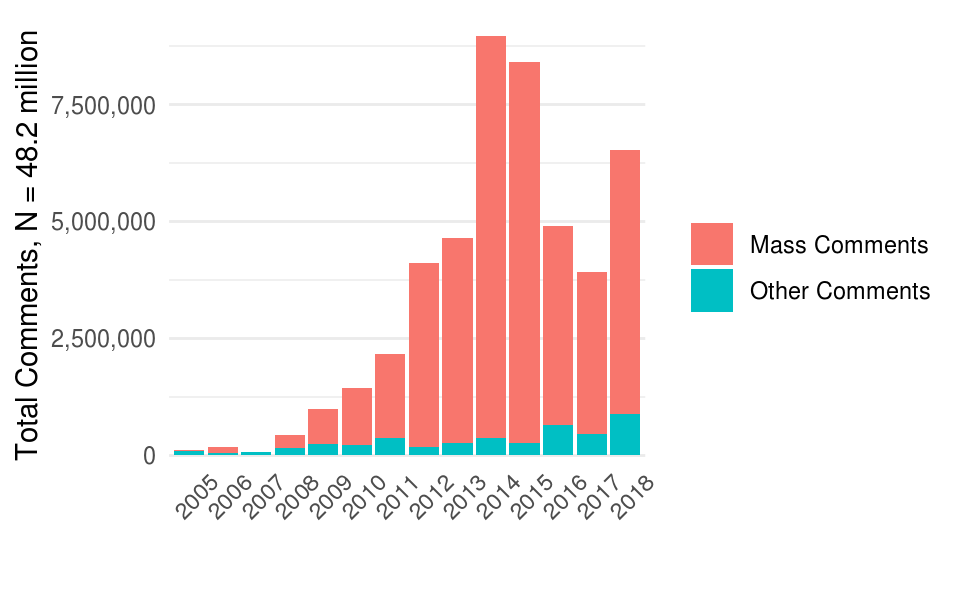
\includegraphics[height =2in]{Figs/comments-mass-vs-unique-1.png}
    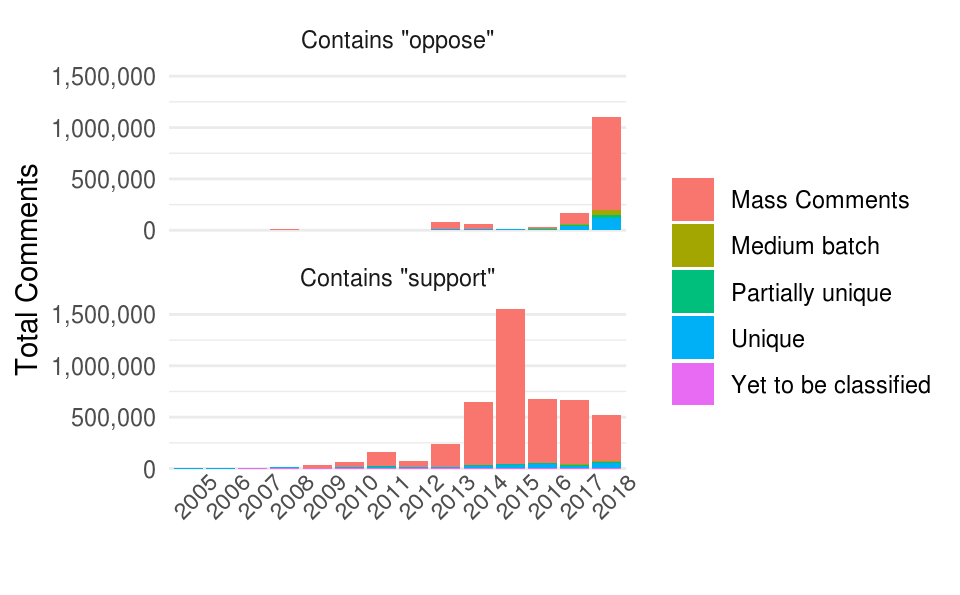
\includegraphics[height =2in]{Figs/comments-mass-support-vs-oppose-1.png}

    \label{fig:comments-mass}
\end{figure}

The right pane of \ref{fig:comments-mass} shows results from a sample of several million comments for which I have digitized the texts. Many of these comments are in support proposed agency rules, as was the case with both the do not call and mercury rule examples. A rough measure of support (whether the comment text includes the word `` support '' or `` oppose '') shows that many more comments mention support, until 2018, when there is a fairly dramatic reversal in the share of comments mentioning `` support '' compared to those mentioning ` `oppose '' (figure \ref{fig:comments-mass}). 





% 
% MEASUREMENT  2
To assess the hypothesis that mass engagement affects the engagement of political principals, I examine the relationship between mass commenting and the behavior of Members of Congress, while attempting to control for other reasons that Members of Congress may comment on a proposed rule. The bold arrow in figure \ref{fig:causal-principals-test} indicates the key relationship in this step.

\begin{figure}[h!]
    \centering
    \caption{Modeling the Relationship between Mass Engagement and Political Oversight}
    \label{fig:causal-principals-test}
\tiny
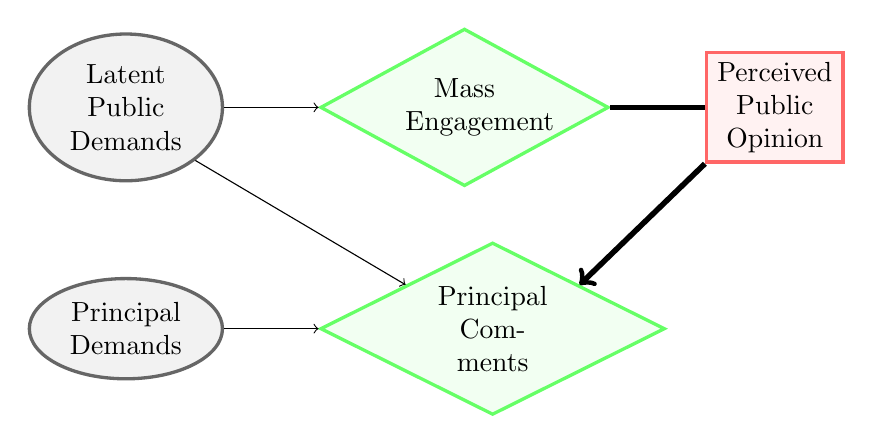
\begin{tikzpicture}[%
    node distance=1.2cm,
    auto,
    text width=1.5cm,
dnode/.style={diamond, align=center, aspect=2, fill=green!5,draw=green!60, very thick, minimum size=2cm},
squarednode/.style={rectangle, align=center, aspect=1, draw=red!60, fill=red!5, very thick, minimum size=1cm},
pnode/.style={ellipse, align=center, aspect=1, draw=black!60, fill=black!5, very thick, minimum size=1cm},
title/.style={rectangle, align=center, aspect=1, minimum size=2cm}
]

% principal nodes 
\node[pnode]        (principaldemands) {Principal Demands};

\node[dnode]      (principaldecides) [right=of principaldemands] {Principal Comments};


% public Nodes
\node[pnode]        (publicdemands) [above=of principaldemands] {Latent Public Demands};

\node[dnode]      (publicdecides) [right=of publicdemands] {Mass\\ Engagement};

% political info
% \node[text centered]      (mobilization) [above=of publicdecides] {Mass\\Mobilization};

% \node[text centered]      (mobilization2) [right=of mobilization] {};

% \node[rectangle, minimum width =3cm, minimum height = 6.8cm, draw=red!60, fill=red!5, very thick]      (politicalinfo) [below=of mobilization2] {};

% \node[text centered]      (politicalinfotext) [below=of mobilization2] {Political Information};

% info
\node[squarednode]      (publicinfo) [right=of publicdecides] {Perceived Public Opinion};
% \node[squarednode]      (principalinfo) [right=of principaldecides] {Perceived Political Consequences};
% \node[squarednode]      (principalinfo2) [below=of principalinfo] {Perceived Principal Opinion};


% \draw[->] (mobilization.south) -- (publicdecides.north);


% public Lines
% \draw[->] (draft.east) -- (publicdemands.west);
\draw[->] (publicdemands.east) -- (publicdecides.west);
\draw[-, line width=2] (publicdecides.east) -- (publicinfo.west);




% principal Lines
% \draw[->] (draft.east) -- (principaldemands.west);
\draw[->] (principaldemands.east) -- (principaldecides.west);
\draw[->, line width=2] (publicinfo.south west) -- (principaldecides.north east);
% \draw[->] (principaldecides.east) -- (principalinfo.west);
% \draw[->] (principaldecides.south east) -- (principalinfo2.north west);
\draw[->] (publicdemands.south east) -- (principaldecides.north west);

% policy 
% \node[dnode]      (policy)       [right=of principalinfo] {Policy Response};
% \draw[->] (politicalinfo.east) -- (policy.west);

\end{tikzpicture}
\end{figure}
\normalsize

I measure the dependent variables, legislator attention and support, several ways. First, I count the number of times Members of Congress engage the agency across rules and before, during, and after comment periods on rules where lobbying organizations did and did not go public. By engaging the agency, I mean that Members of Congress raise a rule in hearings, committee reports, and personal letters that members send to the agency. 
Next, I use text analysis to compare the sentiment and rhetoric used by legislators to that used by each coalition.% Members of Congress may raise agency rules in oversight hearings, reports attached to each agency's budget appropriation, and in personal letters addressed to agency officials. %Using text reuse methods I identify when policy issues raised in draft rules and rule comments attract positive or negative attention from legislators.
Using texts has several major advantages over other measures of congressional attention and sentiment such as partisanship \citep{Yaver2016, Lewis2008}, changes in budget size, or the length of appropriations reports \citep{Bolton2015}. Unlike partisanship, it is issue-specific and does not require assumptions about agency partisanship. While budget changes may reflect real costs, the many reasons that budgets change make it difficult to attribute changes to particular agency actions. The length of appropriations subcommittee reports may indicate the amount of attention committees pay to an agency but they do not vary significantly over time and do not indicate whether committee attention is positive or negative.

Specifically, dependent variables include:

% Similarly, I asses the involvement of presidential appointees and the President's Office of Management and Budget before and after public comment, again comparing rules that were and were not targeted by a campaign (a difference-in-difference). 
% As a validity check, I also look for remarks by elected officials and judges on the level of public engagement.\footnote{
% I expect courts to be more likely to cite the procedural legitimacy of notice comment rulemaking when ruling in favor of public interest group that went public, and less likely to do so when ruling against them, compared to cases where rules received few comments. For example, citing the procedural legitimacy of rulemaking in Vermont Yankee v. NRDC (1978), Justice Rehnquist noted ``More than 40 individuals and organizations representing a wide variety of interests submitted written comments.'' I have collected data, including mentions of public comments, on all Supreme Court cases reviewing agency rules since 1984 and will do the same for a sample of D.C. circuit cases. While I focus on elected officials because they are more likely to respond to mass engagement, courts are also important political principals who explicitly review the legitimacy of rulemaking processes.
\begin{quote}
%\textbf{Dependent variables}

Model 1) Comments from Members of Congress on the rule (total, those mentioning mass comments, and those mentioning organizations in the coalition), Each  $\sim$ zero-inflated negative binomial. 

Model 2) Share of mentions supporting the coalition,  $\sim$  beta. 

Model 3) Rhetorical similarity between comments from the coalition and Members of Congress. 
\end{quote}

Dependent variables 1-2 are one observation per coalition per rule. Model 3 is one observation per comment from a Member of Congress. The key explanatory variables of interest are the measures of mass engagement created in step 1 (how many and what types of comments). One challenge will be controlling for rule salience, which may affect both public and legislator attention (indeed, both are endogenous to rule salience). Another challenge will be controlling for latent public opinion, which may often, but not exclusively, be revealed to legislators through mass engagement.% In addition to cross-sectional analysis, I use a difference-in-difference design within members on rules where groups do and do not go public.

%I examine the relationship between mass engagement and another key variable in agency decisions, political oversight. % other key features of agencies' decisionmaking environments. 
% Do mass comment campaigns indicate that elected officials will be more involved in a rulemaking? 
% Do they indicate a greater chance of a rule being challenged or overturned in court?
% Dependent variables include political principals' attention, positions, and rhetoric, which I measure several ways across rules and within policy areas before and after mobilization campaigns.
% THEORY 2
% Accountability to Congress, the president, and courts have long been central concerns for bureaucracy scholars \citep{Wilson1989}. 
 % Elected officials, political appointees, and judges may also see it as their job to hold agencies accountable to the public will. On the other hand, elected officials often serve private interests,  such as campaign donors, especially when there is little risk of being held publicly accountable themselves.


% To assess the direct influence pathway, I estimate the extent to which mass mobilization around bureaucratic actions makes members of Congress or White House officials more likely to engage or react and whether such mass mobilizations is salient in subsequent litigation. 

 

% [President and Secretary]

% There are two ways to assess the courts as an indirect pathway where mobilization leads to influence. First, mass mobilization may increase the credibility of the threat of litigation. Second mass mobilization may influence the outcome of subsequent court cases over the rule. Both are difficult to measure. The first I measure with a combination of the litigation history of mobilizing groups and specific references to litigation in the comments. The second I assess by identifying instances where courts reference the number or direction of comments or other forms of protest in their decisions and compare rules to the rules under consideration in those cases. While this is rare, legal scholars have noted that " If the validity of a final regulation is challenged in court, the court's review will be based in significant part on how well the agency responded to the public's comments"  (Wagner 1995).
% 

% MEASUREMENT 3 % FIX THIS 
% it is difficult
The main dependent variable here is changes in rule text. However assessing policy change is difficult. Thus, I also use other measures of agency responses to lobbying efforts. 
%Different inputs may yield different results: 
Agencies may or may not change draft policies or may speed up or delay finalizing them. They write lengthy justifications of their decisions in response to some demands but not others. They may or may not extend the comment period. Measuring actual changes in policy text is more difficult. I aim to use automated methods to systemically identify changes between draft and final rules, parse these textual differences to identify meaningful policy changes, and compare them to demands raised in comments to measure which coalition got their way.
Observing policy influence, especially in the final stages of policymaking is difficult. Given the momentum of political agendas and the fact that much is determined before draft rules are made public, changes are often on the margins. But such marginal victories are also the aim of business and other interest groups. 
Additionally, my theory suggests that influence is likely only in cases where mass mobilization is (1) aimed at influencing policy and (2) not accurately anticipated by policymakers. Measuring these will also be difficult.

\begin{figure}[h!]
    \centering
    \caption{Modeling the Relationship between Political Information and Policy Change}
    \label{fig:causal-influence-test}
\tiny
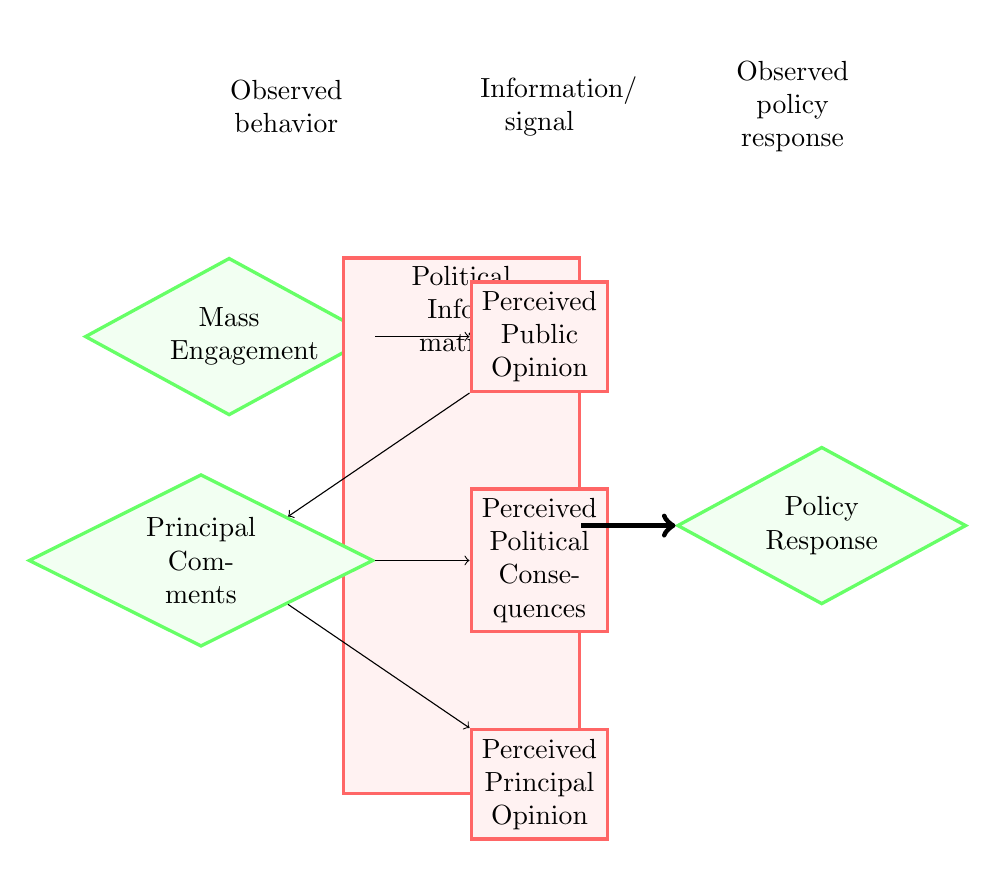
\begin{tikzpicture}[%
    node distance=1.2cm,
    auto,
    text width=1.5cm,
dnode/.style={diamond, align=center, aspect=2, fill=green!5,draw=green!60, very thick, minimum size=2cm},
squarednode/.style={rectangle, align=center, aspect=1, draw=red!60, fill=red!5, very thick, minimum size=1cm},
pnode/.style={ellipse, align=center, aspect=1, draw=black!60, fill=black!5, very thick, minimum size=1cm},
title/.style={rectangle, align=center, aspect=1, minimum size=2cm}
]


% \draw[->] (publicinfo.east) -- (policy.west);
% \draw[->] (principalinfo.east) -- (policy.south);
% \draw[->] (principalinfo2.east) -- (policy.south);



% public Nodes
\node[dnode]      (publicdecides)  {Mass\\ Engagement};


% political info
\node[text centered]      (mobilization) [above=of publicdecides] {};

\node[text centered]      (mobilization2) [right=of mobilization] {};

\node[rectangle, minimum width =3cm, minimum height = 6.8cm, draw=red!60, fill=red!5, very thick]      (politicalinfo) [below=of mobilization2] {};

\node[text centered]      (politicalinfotext) [below=of mobilization2] {Political Information};

% info
\node[squarednode]      (publicinfo) [right=of publicdecides] {Perceived Public Opinion};
\node[squarednode]      (principalinfo) [below=of publicinfo] {Perceived Political Consequences};
\node[squarednode]      (principalinfo2) [below=of principalinfo] {Perceived Principal Opinion};

% principal Nodes
\node[dnode]      (principaldecides) [left=of principalinfo] {Principal Comments};



% public Lines
\draw[->] (publicdecides.east) -- (publicinfo.west);




% principal Lines
\draw[->] (publicinfo.south west) -- (principaldecides.north east);
\draw[->] (principaldecides.east) -- (principalinfo.west);
\draw[->] (principaldecides.south east) -- (principalinfo2.north west);

% policy 
\node[dnode]      (policy)       [right=of politicalinfo] {Policy Response};
\draw[->, line width = 2] (politicalinfo.east) -- (policy.west);


% Titles
% \node[title]      (1) [above=of draft] {Policy};
%\node[title]      (2) [above=of groupdemands] {Preferences};
\node[title]      (infotitle) [above=of publicinfo] {Information/ signal};
\node[title]      (3) [left=of infotitle] {Observed behavior};
\node[title]      (5) [right=of infotitle] {Observed policy response};

\end{tikzpicture}
\end{figure}
\normalsize

Observational studies of policy decisions are almost always frustrated by the fact that decisionmakers rationally anticipate the actions of those who would influence them, rendering this influence difficult to observe. Thus I expect to observe larger effects in cases where mobilization or the level of engagement achieved was not anticipated by agency staff. However, as long as rulewriters do not perfectly anticipate mass engagement, it should have observable, if depressed, effects. 

My method of identifying whether a rule seems to move in the direction requested is similar to leading existing methods---\citet{Yackee2006JOP} measure whether commenters requested for more or less regulation---and superior to self-reported influence \citep{Furlong1997}.

I aim to discover latent coalitions by textual similarity (having removed all sentences quoting the agency's draft rule and call for comments), parse policy demands, and estimate relative probabilities that a policy change favors a given coalition. I then model the relationship between my measures of policy success and coalition size, intensity, and contagion and assess mechanisms
%---indirect-strategic, direct-normative, indirect-normative---
by which political information may influence agency decisions.

Most rules address long-defined problems. They are next steps advancing a policy agenda \citep{West2013} or the first steps in a new, often reverse, policy direction, it is possible that effects of ``going public'' are cumulative in a policy area over time, starting out small, but gaining agenda-setting power with sustained public attention. This may not be possible to measure with the rule-focused research design outlined above. However, if sequential rules can be linked to distinct policy agendas, my strategy could be extended to model dynamics over time following \citet{Brookhart2015}.



% Measuring Policy Change}
% Policies may shape and be shaped by many forces, including the collective action of citizens, expert opinions, and businesses interests. Yet the drivers and consequences of policymaking are difficult to disentangle. Business groups may fund scientists or advocacy campaigns to preempt or undo costly regulations. Experts and policymakers may inspire broader civic mobilization, and citizen mobilization may, in turn, shape the priorities of experts and policymakers. Some policy debates divide along lines of citizen and corporate interest or expert and popular opinion, but many entail various clusters of claims regarding the public interest, expertise, and business interests: claims about the public good, scientific truths, and the proper role of government. Inferring policy demands from identity alone and assuming static coalitions may miss much of the story. 

\paragraph{Text as Data}
Existing measures of who gets their way in rulemaking are blunt---hand-coding texts on a few pre-defined and simplified categories such as ``pro- or anti-regulation.'' This is well motivated by theory, but in practice, it is often unclear whether a policy, on its face, increases or decreases government regulation.%, is liberal or conservative, or maps on to any other such latent dimension. 
Another drawback of the hand-coding approach is that one must often read each comment and compare it to the rule change to identify influential groups. %If groups get their way when they lobby in many venues over time or on obscure or uncontested rules, studies focusing on highly visible and contested policy processes may miss much. Conversely, if mass mobilization in high-profile and hotly-contested rules matters, studies of rulemaking that discard the hundreds of thousands of form letters and other evidence of occasional bursts of civic engagement are unable to assess if mass participation matters. Legal scholarship suggests that mass mobilization may be important (Coglianese 2001). This limited and potentially biased empirical focus is largely due to the cost of hand-coding methods.

I use computational text-analysis tools to address these concerns. Political scientists have only begun to leverage text-analysis tools to measure political relationships (see Grimmer 2013 on priorities, Kl\"uver and Mahoney 2015 on framing, Wilkerson et al. 2015 on tracing policy ideas). I expand analysis of rulemaking from thousands of documents to hundreds of thousands and from a few variables to many. %Specifically, text-analysis tools can do two things: (1) rapidly code large amounts of text for pre-established theoretically-informed variables and (2) identify new dimensions of variation (Grimmer and King 2011). A key advantage of text-analysis methods is that they can identify new dimensions of variation one had no prior reason to suspect, suggesting new hypotheses. For example, in addition to our prior notions of who ought to be influential, we may expect that the topics, priorities, arguments, or issue frames on which comments cluster may identify new dimensions distinguishing winning and losing coalitions in different contexts.  %The literature suggests three broad rival hypotheses: \textit{The change between the draft and final rule reflects the interests of ($H_1$) underrepresented groups, ($H_2$) regulated businesses, ($H_3$) no particular class of commenters.} 
% regs.gov
% regulation.gov - sometimes they are coming in after the time period

%I refine tools to measure influence in policymaking with two aims: (1) to estimate the relative influence of different actors or texts and (2) to identify new factors that predict influence. These methods will allow new tests to advance core debates about how and why influence occurs and may benefit a wide range of scholarship. Active debates over bureaucratic autonomy and capture (Carpenter 2001, 2010, Carpenter and Moss 2014) and the influence of Congress (Clinton et al. 2014, Farhang and Yaver 2015), the courts (Lauderdale and Clark 2014), the president (Carrigan and Krazdin 2015), and public opinion (Dunleavy 2013) will all benefit from using text-analysis to measure influence. 

%Generally speaking, my method of measuring influence in each rulemaking case has two steps, each targeting a conceptually distinct type of influence. First I identify the major dimensions of variation in comments and the direction in which the policy moved in relation to those dimensions, i.e. which side(s) won. Second, I identify particularly influential texts within the winning coalition(s). 

% More specifically, to address my three descriptive questions, I propose to uses an ensemble of five text-analysis methods to identify participants, track coalitions, and quantify the relationship between various input texts and outcome text. This ensemble combines (1) citations(finding texts that mention the same organization and individual names across comments) to identify participants (2) single member topic modeling to identify coalitions, (3) Smith-Waterman alignment (text reuse) identify text fragments copied from each individual texts, (4) mixed-member topic models to identify the distribution of topics in comments and changes to rule texts, and (5) sentiment analysis to identify positive and negative positions on each topic. These are described in more detail below.

%This ensemble method has several applications in this project. First, it allows me to identify clusters (possible coalitions) of actors commenting on draft regulations and estimate the relative alignment of each of these clusters (and individual documents within them) to the draft rule and final rule. Similarly, it allows me to identify clusters of actors submitting briefs to courts reviewing these rules and their alignment with the court opinion. 

%In the remainder of this section I describe what is measured by each component of the ensemble, and then discuss how these improved measures of who participate, who lobbies together, and whose ideas end up in policy through rulemaking can provide leverage to test mechanisms of policy feedback. 



\paragraph{Measuring Policy Change}
%\subsection{What Policy Texts Do?}

As described below, I measure the extent to which the text of a policy becomes more similar or less similar to the text of each public comment. 

One way to think about this is that this change represents an increase in utility for those lobbying for the change. Purposeful actors got what they asked for and presumably reap the rewards. All dimensions of disagreement collapse to the latent dimension of utility. Actors participate and form coalitions to the extent that the expected benefits exceed the costs of doing so. Each new layer of law affects politics by altering actors' utility functions. 

Taking a broader view of politics offers a less parsimonious, but more direct interpretation. Changes in law may deliver utility, but more precisely they reflect ideas. These may be ideas about ``who gets what, when, and how,'' but also about identities, aspirations, possibilities, whose opinions matter, and who constitutes the political community, which may be difficult to reduce to a single dimension. Focusing on costs and benefits or alone, risks overlooking much of the ideological and interpretive work lawmaking does in constructing political communities, possibilities, and norms. Public comments in rulemaking, like other forms of policymaking, may often be about more than self-interest. 

% Indeed ``who succeeds?'' is a constraining question laden with certain ideas of what politics really is or ought to be. A better question may be ``How do certain ideas end up in law and how has this shaped politics and law over time?'' This latter formulation recognizes that ideas may end up in law as accidental to other efforts and that politics is not only who gets what but, more fundamentally, a process of deciding who we are and what we want to do together. 

% In the case of rulemaking, each notice-and-comment process creates an implicit political community based on who participates and whose interests are claimed to be represented. Regulations generally prescribe concrete rights, prohibitions, and governmental actions, making clear what was decided to be done. They also establish norms, issue frames, scientific and legal standards, and goals that inspire and constrain politics in other policy processes, especially future rulemakings on the same issue.

% Importantly, few observers would see any final rule as the final word. Rules are frequently revisited at regular intervals, challenged in court, rewritten under future administrations, rebuked by a new Congress, and occasionally swept aside by new legislation. Most often, the questions in rulemaking will be revisited by the same agency and many of the same participants, but they are not the same; both have been transformed and engage the questions on terrain reshaped by added layers of law. This means that it is essential to consider the historically contingent evolution of policy and lobbying coalitions over time. Quantitative scholarship on rulemaking rarely considers the date rules are made, much less how the politics of rulemaking may be historically contingent. I aim to address this gap. 

% One way to think about the kind of political influence I aim to study is to ...

%Recognizing this, I try to ....
% \paragraph{Measuring change in policy texts}

% If available and reliably reflecting what actors want, policy positions expressed as texts have great advantages over those expressed in votes.

Policy disagreements are disagreements about words that give governmental force to ideas. Information is an important currency for those trying to influence policy and that rhetoric and framing can affect perceptions of facts and policies. Policy learning can be seen as an updating of where one stands, an updating of beliefs about the what is true about the world and, most specifically, an updating about which words (and thus ideas) ought to be in law. Importantly, policymakers are constantly learning about new problems, facts, and policy ideas about which they had no prior position. Thus new dimensions of disagreement are created every time claims are advanced about new problem definitions, new facts, and new ideas for what the law ought to say.

Estimating spatial ideal points is a leading way of estimating what actors want, especially when we only observe a series of votes. The quantity of interest is what kind of policy actors ideally want, and because voting only tells us whether one is for or against a policy text, we need multiple observations in which an actor (or others who plausibly share their position) falls on each side to begin to narrow down their ideological distance from any given policy. To get multiple observations, we must assume that a number of proposed policies can be placed as different points on the same underlying dimension of disagreement. When it is persuasively argued that a number of these underlying issue dimensions more or less collapse to an even more general dimension, we further increase our observations and thus the information we have about each actor regarding that more general dimension. 

When, rather than up or down votes, we have the text of what each actor wanted, we have much more information about where they stand in relation to a policy text. Indeed, instead of needing to uncover more general latent dimensions and estimate actors' positions on them, we directly observe the quantity of interest: the substance, direction, and magnitude of the disagreement in each case. We can cluster these disagreements to make more general statements about the broader nature of disagreements and relative policy potions, but, unlike with voting data, this reduction is not necessary to know the extent to which actors are getting what they want as we can directly observe how much outcome texts incorporate various actors' expressed ideal language. Flattening proposed changes in texts to \textit{n} dimensions where \textit{n} is fewer than the number of unique demands made by all actors may help descriptively, but is not required analytically. For example, we may reduce textual policy demands to left and right ideologies or preferences for more or less government, and doing so can be descriptively useful, but it is neither necessary nor helpful for answering the question of whose ideas end up in law.

Importantly, my project does not attempt to answer what actors want in general, \textit{a priori} of any policy proposal. Without some reference point (existing policy, for example) what actors want may be impossible to define. I assess what commenters want \textit{given} a proposed policy. What commenters request may not be a sincere representation of their ideal policy, but it is plausibly what they really want given what they believe is possible. While this may be insufficient for estimating ideal points, it is sufficient for measuring who gets what they ask for. 

If the primary aim is to identify policy actors' ideological proximity to each other, the analysis can be reduced to the similarity and difference in their ideal policy texts, summed across all areas or within broad policy areas. If alternatively, we ask whose ideas end up in policy, we want to know how similar the policy outcome was to the specific suggestions of each actor and the frequency of changes in their proposed direction.% regardless of whether they are advocating for ideologically consistent, orthogonal, or even opposite positions in different cases. In practice, the unique dimensions of disagreement in each policy process are rarely perfectly parallel or orthogonal. Mapping ideological distance requires reducing to some tractable number of dimensions. Measuring rates of getting one's way do not.
%This is one great advantage of textual data compared to votes. Each observation is far richer in content and analysis requires fewer assumptions to say where actors really stand on a proposed policy. 
A finding that the words one actor suggested be added to a policy were twice as likely to appear in the final policy as average is a powerful and intuitive description of where power to shape policy resides.\footnote{This is, perhaps, even more powerful than saying that the policy tended to shift toward their ideal point on some latent dimension, where the exact content anchoring the ideal point and the dimension are at least slightly ambiguous.}

\paragraph{Measuring the extent commenters got what they asked for}

Participants may ask for two general kinds of things: they ask for specific changes to identified parts of the text or they may ask for a broad shift in emphasis, what \citet{Jones2005} call a policy image. For example, on the same Clean Power Plan rule, some may ask the Environmental Protection Agency to make specific changes to two sentences having to do with the classification of power plants.% and the division of federal and state enforcement authority. 
Others may ask for broad reframing to focus less on economic costs and more on environmental equity and the effects of pollution on children \citep{Rinfret2011}. Many commenters do both. 
I thus collect two key pieces of information from the rulemaking record: the text comments and the change from the draft rule to the final. %I use each type of information in a different kind of analysis, one targeting specific demands and one targeting broad demands. 
Both approaches require the same initial steps. To identify how exactly the rule changed from draft to final, I use text reuse methods to identify what is the same and has been added or subtracted. 
%Similarly, I identify text in comments that is not copied from the draft rule.\footnote{I may also need to exclude other kinds of text such as narratives introducing the commenter which commonly precede policy demands.} 
The result of these two steps is the changes requested by commenters and textual change in the rule. 

To identify the adoption of specific demands, I use the same text reuse methods to identify any matches between textual changes in the rule and the changes requested by commenters. If final rules include the specific phrases suggested in comments, this is evidence that these commenters got some of what they asked for. The significance of this kind of relationship between texts could be measured by how many words were copied, weighted by the forcefulness of these words. For example, I could create a dictionary of legally-significant words such as ``shall,’’ ``must,’’ ``enforcement,’’ and ``standard.’’ and weight textual alignment scores accordingly. Text reuse can be measured for individual commenters and averaged over coalitions. 

To identify the adoption of demands for broader shifts in policy image and emphasis, I propose a relational topic modeling approach. In contrast to the single topic model used to classify commenters into coalitions, this approach assumes that each text is a mixture over a number of topics. Each word token in a document is assigned to exactly one topic. Words and thus documents have distributions over topics. The extent to which distribution of topics that changed from the draft to the final is similar to the distribution in comments may be seen as a measure of whether the commenter got what the kind of change in policy emphasis they asked for.\footnote{
% anprm footnote 
Some rulemaking processes also have a commenting period before the draft policy is published. In these cases, commenters respond to an Advanced Notice of Proposed Rulemaking (ANPRM). A similar approach can be used in these processes with the key difference that similarities between comments and the draft rule (now the outcome text), either in specific text fragments or general topic distribution, take on a different meaning. Instead of representing changes to a policy text, it may represent common understandings of what policy already was or had to be on this topic. Changes in the final rule more plausibly represent differences in what policy could be. With respect to the ANPRM and proposed rule, it is more difficult to infer that the same result would not have occurred without their comments. While such counterfactual inference is not my purpose and both measure the same core phenomena of the words actors want becoming policy, interpretation of what this means must attend to this difference.}

\paragraph{Relating comments to overall rule changes}

Next I combine topic modeling approaches with text reuse methods, allowing better measurement not just of what is discussed but the topic distributions of what is being added, cut, copied, or otherwise receiving special attention. 
%I call this a relational topic modeling approach. 
Of course, all topic models focus on the relationship between text, but by making some of the text units themselves a relationship between texts with text reuse methods, the topic model takes a ``difference in difference'' (e.g. what was added or deleted) % or ``difference in similarity'' (e.g. what was copied) 
form. Much of the rule content is retained from one version to the next, but some content changes. We want to know how these changes relate to the changes proposed by sophisticated comments. 

%\subsubsection{LDA: the Distribution of Words over Topics} 

% This section first reviews the \textit{Latent Dirichlet Allocation} (LDA: Blei et al. 2003) model, then the unique text preparation and effect estimation steps necessary to address my questions, and finally additional steps and extensions to improve topic and effect estimation. In the discussion section, I suggest additional questions that may be addressed using the text analysis approach advanced here.

To measure the relationship between comments and policy change, I draw on the \textit{Latent Dirichlet Allocation} (LDA: Blei et al. 2003) model. Unlike the model used to estimate coalition membership, this is a mixed-member model. In LDA, each document can be represented as a vector of topic proportions, i.e. what fraction of the words in that document belong to each topic (Blei et al. 2003). For example, in a model of a rulemaking under the Environmental Protection Agency's Clean Power Plan, ``climate,'' ``adaptation,'' ``carbon,'' and a dozen other words may co-occur and indicate a topic about climate change. The words, ``clean'', ``air,'' and ``health'' may also co-occur and have relatively high frequencies in a topic that seems to be about air quality.  The change in the rule from NPRM to Final Rule and each comment would have a $\pi$ proportion of words belonging to the \textit{climate change} topic (\%$\tau_{Climate}=\pi_{Climate}$). This may be a relatively high portion for Climate Action Coalition comments and a low portion for American Lung Association comments ($\pi_{Climate, CAC} > \pi_{Climate, ALA}$) compared to the air quality topic, which may be the opposite ($\pi_{AirQuality, CAC} < \pi_{AirQuality, ALA}$). If the rule changes to focus more on climate change from draft to final rule ($\pi_{Climate, \Delta EPA} > \pi_{AirQuality, \Delta EPA}$), the Climate Action Coalition may be seen as more successful than the American Lung Association with respect to the broad emphasis of the regulation. This offers a new way to capture what Jones and Baumgartner (2005) call \textit{attention allocation}, the changing weights on policy images and issues: in this case, what the Environmental Protection Agency ought to do.

\begin{figure}[h!]
\label{percent}
\caption{The Latent Dirichlet Model (LDA)}
\begin{tabular}{@{\extracolsep{5pt}}rlccl} 
& & & \\
Text: &\fbox{Comments} &  $\longrightarrow$ & \fbox{Change in Rule}\\
& & & \\
Dist. over $T$ topics (e.g. $\tau_{1:3}$): & Comment$_{j_1}$ $\sim $\{\%$\tau_{1}$, \%$\tau_{2}$, \%$\tau_{3}$\}  & & $\Delta$Rule $\sim $\{\%$\tau_{1}$, \%$\tau_{2}$, \%$\tau_{3}$\}\\
& Comment$_{j_2} \sim $\{\%$\tau_{1}$, \%$\tau_{2}$, \%$\tau_{3}$\} & & \\%$\Delta$Rule$-$ $\sim $\{\%$\tau_{1}$, \%$\tau_{2}$, \%$\tau_{3}$\}\\
& Coalition$_{(j_1+j_2)} \sim $\{\%$\tau_{1}$, \%$\tau_{2}$, \%$\tau_{3}$\} & &
\end{tabular}
\end{figure}


% For comment $j$ and rule change $\Delta r$ on topics $\tau_{1:T}$ with proportions $\pi_{j}$ and $\pi_{\Delta r}$:
% \begin{align*}
% Success_{j, \tau} \ &= 1-(\pi_{j, \tau} - \pi_{\Delta r,\tau})\\
% \end{align*}

I focus on draft-to-final rule change by selecting only the text that was added or subtracted. This can be thought of as a versioning problem where the agency updates the rule. To focus on what changed, I excluded sentences that appear verbatim in the NPRM. I use the Smith-Waterman alignment algorithm (developed for identifying DNA matches and commonly used in plagiarism software) to identify sections of text that are close matches. Wilkerson (2015) successfully employs this approach to identify content copied from various bills in the legislative processes leading to the Affordable Care Act.


%More precisely, this includes the topic distribution of text added to the rule $\pi_{\Delta r+}$ and subtracted $\pi_{\Delta r-}$:
%\begin{align*}
%Success_{j, \tau} \ &= 1-(\pi_{j, \tau} - \pi_{\Delta r+,\tau}) +  1-(\pi_{j, \tau} - \pi_{\Delta r-,\tau})\\
%\end{align*}



The percent of each topic $\tau$ within each document $j$ is estimated as $\pi_{j, \tau}$ where:
\begin{align*}
%z_i &\sim Multinomial(\theta_{D_{i, j} })\\
%\theta_k &\sim Dirichlet(\alpha)\\
%w_i &\sim Multinomial(\phi_i)\\
%\phi &\sim Dirichlet(\beta) \\
%=\\
\tau_{i, j} | W_{i, j} &\sim Multinomial(\pi_{w_{i, j} })\\
\pi_{j} &\sim Dirichlet(\alpha) \\ % should tau be there
W_{i, j} &\sim Multinomial(\rho_{\tau,w})\\ % should be W_{tao}, probability of drawing a word in W at token i is drawn from a multi distribution of the probabilities that each word is in each topic
% should be rho_{w, tau}
\rho_{\tau,w} &\sim Dirichlet(\beta) 
\end{align*}

We observe the total number of unique words ($w_1,...,w_W$) in the vocabulary of all documents and $w_{i, j}$ is the word observed at the $i$th token in document $j$. All texts are ``tokenized'' by giving each word\footnote{For topic estimation, I use single words, but tokenizing may be done by sentence or by any n-gram string of characters or words.} a unique index $i$. If token $i$ belongs to topic $\tau$, then the probability that the token is word $w$ is the topic-specific probability $\pi_{\tau, w}$. At the document level, $\pi_{\tau, j}$ %/$\theta_{i, k}$ 
is the estimated proportion of topic $\tau$ for document $j$. %, a $i$ x $\tau$ matrix of the proportion of words from each topic in each document. 

$T$, $\alpha$, and $\beta$ are defined. 
$T$ is the number of topics $(\tau_1,...\tau_T)$ where $\tau_{i, j}$ is the topic of the $i$th token in document $j$. Each token comes from exactly one topic.
$\alpha$ is the parameter of the prior on the per-document topic distributions, and
$\beta$ is the parameter of the prior on the per-topic word distributions. 
$\rho_{\tau, w}$ % / $\phi_{w, k}] / $ 
is the distribution over $w$ words in each topic $\tau$, i.e. the probability of drawing the $w$th word of the vocabulary for topic $\tau$.
%$\rho_{j,w}$ is the probability that the $i$th token of document $j$ lies in
%$\tau_{i, j}$ %/D
%, $\pi_{w_{i, j}}$.%$\theta_{D_{i, j}}$ / is this right?

%w / $\psi$ is the specific word (the only observable variable) 
% CHOOSE A WORD w[i] GIVEN THE TOPIC z

The result is a quantitative measure of the alignment between suggestions made in comments and text added or subtracted from the draft to final rule. A similar approach can estimate the relationship between ANPRM comments and the draft rule text, omitting the draft-to-final text reuse step. Credible intervals for these comment and topic-specific alignment scores can be calculated from posterior distributions. 

% \subsection{Measuring the Role of Agency Missions and Reputations in Decision making}

% \subsubsection{Measuring agency reputations}

% \subsubsection{Linking comments and reputations

% Chapter 3 Results - Why So Much Mail?

% Chapter 4 Results - Influence on Principals

% Chapter 5 Results - Influence on Agency Policymaking

% Chapter 6 Environmental Justice Case Study
% \section{Case Study: Environmental Justice in Rulemaking} 
This chapter 
explores the role of public comments in rulemaking by focusing on their role in the environmental justice movement. Environmental justice concerns focus on the unequal access to healthy environments and protection from harms caused by things like pollution and climate change. The ways in which agencies consider environmental justice highlights how rulemaking has distributive consequences, how the public comment process creates a political community, and how claims raised by activists are addressed, conditional upon their alignment with agency missions. Examining over 20,000 rulemaking processes at agencies known to address environmental justice concerns, I find that when public comments raise environmental justice concerns, these concerns are more likely to be addressed in the final rule. While we cannot infer that agencies addressing environmental justice concerns is caused by the public comments themselves, comments may be a good proxy for mobilization in general. Furthermore, the correlation between mobilization and policy changes is largest and most significant in agencies with missions focused on environmental and distributional policy, i.e. the kinds of agencies we may expect to be most responsive to environmental justice concerns.

This case illustrates the way that activists use public comments to inject ideas directly into the rulemaking process. I focus on the environmental justice movement because it offers a broad but tractable scope for analysis and shows what is at stake in the politics of rulemaking.  How rules consider environmental justice issues illustrates how rulemaking constructs a political community of ``relevant'' stakeholders and ``appropriate'' criteria to evaluate policy consequences. Thus, the idea of environmental justice is an example of how social movements can mobilize norms and evaluative frameworks that are connected to organizational identities, mission, and reputations and that have implications for bureaucratic decisions. 

The use of an environmental justice frame does not always imply the same communities of concern. Environmental justice emerged out of movements against environmental racism, especially the disposal of toxic substances in communities of color \citep{Bullard1993ConfrontingGrassroots}. However, the term quickly took on a wider array of meanings, encompassing any marginalized group. In 1994 the Bill Clinton signed an Executive order on Environmental Justice that required all parts of the federal government to make ``addressing disproportionately high and adverse human health or environmental effects of programs, policies, and activities on minority populations and low-income populations'' a core aspect of their mission. This meant considering disproportionate effects during rulemaking.

Fundamental definitions of the public good and minority rights are implicit in agency rules. The public comment process offers an opportunity to protest these definitions. Protest is one way that  marginalized groups can communicate opinions on issues to government officials \citep{Gillion2015ProtestDistrict,Gillion2013ThePolicy}. In the case of the EPA's Mercury Rules, two such issues were decisive. First, as with many forms of pollution, mercury-emitting power plants are concentrated in low-income, often non-White communities. Second, certain populations consume much more locally-caught freshwater fish, a major vector of Mercury toxicity. Studies inspired by the political controversy around the Mercury Rules found high risk among communities included ``Hispanic, Vietnamese, and Laotian populations in California and Great Lakes tribal populations (Chippewa and Ojibwe) active on ceded territories around the Great Lakes'' (EPA 2012). Thus the standards that EPA chooses are fundamentally dependent on whom the regulation aims to protect: the average citizen, local residents, or fishing communities. This decision has disparate effects based on race and class because of disparate effects based on geography and different cultural practices. Such disparate impacts are often called environmental justice issues.

In December 2000, when the EPA first announced its intention to regulate Mercury from power plants, the notice published in the Federal Register did not address environmental justice issues such as the disparate effects of mercury on certain populations. Risks were only discussed in reference to ``the U.S. population'' (EPA 2000). When the first draft rule was published, it only discussed the effects of the rule on regulated entities, noting that ``Other types of entities not listed could also be affected'' (EPA 2002). Commenting on this draft, Heather McCausland of the Alaska Community Action on Toxics (ACAT) wrote:
\begin{quotation}
``The amount of methyl-mercury and other bio accumulative chemicals consumed by Alaskans (especially Alaskan Natives) could potentially be much higher than is assumed...The Alaska Native mortality rate for babies which according to the CDC is 70\% higher than the United States average. Indigenous Arctic \& Alaskan Native populations are some of the most polluted populations in the world (http://www.amap.no/). Global transport \& old military sites contaminate us too''
\end{quotation}

After receiving hundreds of thousands of comments and pressure from tribal organizations, a revised proposed rule echoed McCausland's comment noting that ``Some subpopulations in the U.S., such as: Native Americans, Southeast Asian Americans, and lower income subsistence fishers, may rely on fish as a primary source of nutrition and/or for cultural practices. Therefore, they consume larger amounts of fish than the general population and may be at a greater risk of the adverse health effects from Hg due to increased exposure'' (EPA 2004). 

After nearly a million additional public comments, a revised proposed rule ultimately included five pages of analysis of the disparate impacts on "vulnerable populations" including ``African Americans,'' ``Hispanic,'' ``Native American,'' and ``Other and Multi-racial'' groups (EPA 2011). In the final rule, the language of ``vulnerable populations '' was replaced with ``minority, low income, and indigenous populations'' (EPA 2012). EPA had also conducted an analysis of sub-populations with particularly high potential risks exposure due to high rates of fish consumption as well as an additional analysis of the distribution of mortality risk by to race.

Of this second round of comments, over 200 explicitly raised the environmental justice issues. The Little River Band of Ottawa Indians expressed the Tribe's ``frustration at trying to impress upon the EPA the multiple and profound impacts of mercury contamination from a Tribal perspective. Not to mention the obligations under treaties to participate with tribes on a “Government to Government” basis. At present, no such meetings have occurred in any meaningful manner with EPA Region V, the EPA National American Indian Environmental Office, nor the State of Michigan’s Department of Environmental Quality.'' They conclude that "Although EPA purported to consider environmental justice as it developed its “Clean Air Mercury Rule,” it failed utterly. In this rulemaking, EPA perpetuated, rather than ameliorated, a long history of cultural discrimination against tribes and their members'' (Sprague 2011). Did comments like these play a role in EPA's changed analysis of who Mercury limits should aim to protect?

Given the many potential sources of influence, it may be difficult to attribute causal effects of particular comments on a given policy. However, comments may serve as a good proxy for the general mobilization of groups and individuals around an administrative process, and it is not clear why EPA would not address environmental justice in the first draft of a rule and then add it to subsequent drafts in the absence of activists mobilization. Electoral politics does not offer an easy explanation. The notice proposing the Mercury Rule was issued by the Clinton administration, the same administration that issued the Executive Order on Environmental Justice, and the subsequent drafts that did address environmental justice issues were published by the Bush administration, which had a more contentious relationship with environmental justice advocates, while Republicans controlled both houses of Congress. The expansion of the analysis from one draft to the next seems to be in response to activist pressure. 

Mobilization around ideas like environmental justice may even affect policy discourse when agency administrators are explicitly hostile to the cause. For example, in an October 2017 proposed rule to repeal restrictions on power plant pollution, the Trump EPA acknowledges that ``low-income and minority communities located in proximity to [power plants] may have experienced an improvement in air quality as a result of the emissions reductions.'' Because of the Executive Order requires attention to environmental justice and because the Obama EPA discussed it when promulgating the rule, the environmental justice cannot safely be ignored. However,  the Trump EPA contends, the Obama EPA ``did not address lower household energy bills for low-income households [and that] workers losing jobs in regions or occupations with weak labor markets would have been most vulnerable'' (EPA 2017). As of \today, this proposed rule has received over 150,000 public comments. 

Tracing ideas like environmental justice through the rulemaking record may offer one way to study the mechanisms by which social movements do or do not influence bureaucratic policymaking. Specifically, if rules are proposed without attention to environmental justice concerns, but environmental justice concerns are raised in the public comments and then appear in the final policy, this may be evidence that mobilization mattered.

Environmental justice is certainly not the only way to observe such effects, but it has some convenient properties. First, policies framed as ``environmental'' issues are, unlike issues like issues like civil rights and immigration, inconsistently racialized and, unlike issues like taxes and spending, inconsistently focus on \textit{distributions} of costs and benefits. Despite almost always having disparate impacts, an environmental frame often creates a human-environment distinction and shifts attention to non-human objects such as air, water, food, or landscapes and away from the distribution of access to these objects or protection from them when they are contaminated. Second, compared to other ideas around which people mobilize, ``environmental justice'' is a fairly distinctive phrase. Most people who use this phrase share a general definitional foundation. Third, this phrase is fairly common when the idea is being discussed, i.e. there are not many synonyms and groups raising equity concerns on ``environmental'' issues commonly refer to environmental justice.  Many who use the narrower, related term ``environmental racism'' also use ``environmental justice'' in their advocacy.  Finally, the term is relevant to rulemaking records in particular because of an Executive Order issued in 1994 by President Clinton "Federal Actions to Address Environmental Justice in Minority Populations and Low-Income Populations" which required all agency actions and policies to consider environmental justice implications. This does not mean that all draft or final rules do so, but when they do, they tend to cite the executive order and explicitly discuss environmental justice. For the same reason, commenters, especially sophisticated ones, who critique draft rules also use the cite this executive order and use this language. 

 \subsection{Data}
In order to examine whether the environmental justice movement's mass mobilization of letter-writing influences the discourse around policies, I use the text of draft rules, public comments, and final rules retrieved from regulations.gov.  Figure \ref{fig:ej} compares the use of the term ``environmental justice'' in draft policies, public comments on these drafts, and the final versions of the policies. I collected all 58,789 documents from the website regulations.gov that use the phrase ``environmental justice.'' This includes 4,141 notices of intent to propose a rule, 5,109 proposed rules, 17,539 public comments on these notices and proposed rules, and 10,418 final rules. Additionally, I collected all draft and final rules from all 35 agencies that have published at least one rule addressing environmental justice, an additional 40,096 documents.  % CORRECT THESE NUMBERS 

Notably, more than twice as many finalized rules as proposed rules contain the phrase ``environmental justice.'' This suggests a systematic element in how agency policymakers are revising draft rules. Below, I investigate the extent that this change from the draft to final policy is related to environmental justice issues being raised in the public comments. 

\begin{figure}[h!]
\caption{Number of Rules where Environmental Justice Appears in the Record (Left) and Number of Comments per Notice or Proposed Rule (Right). Text indicates the agency for the most commented on rules.}
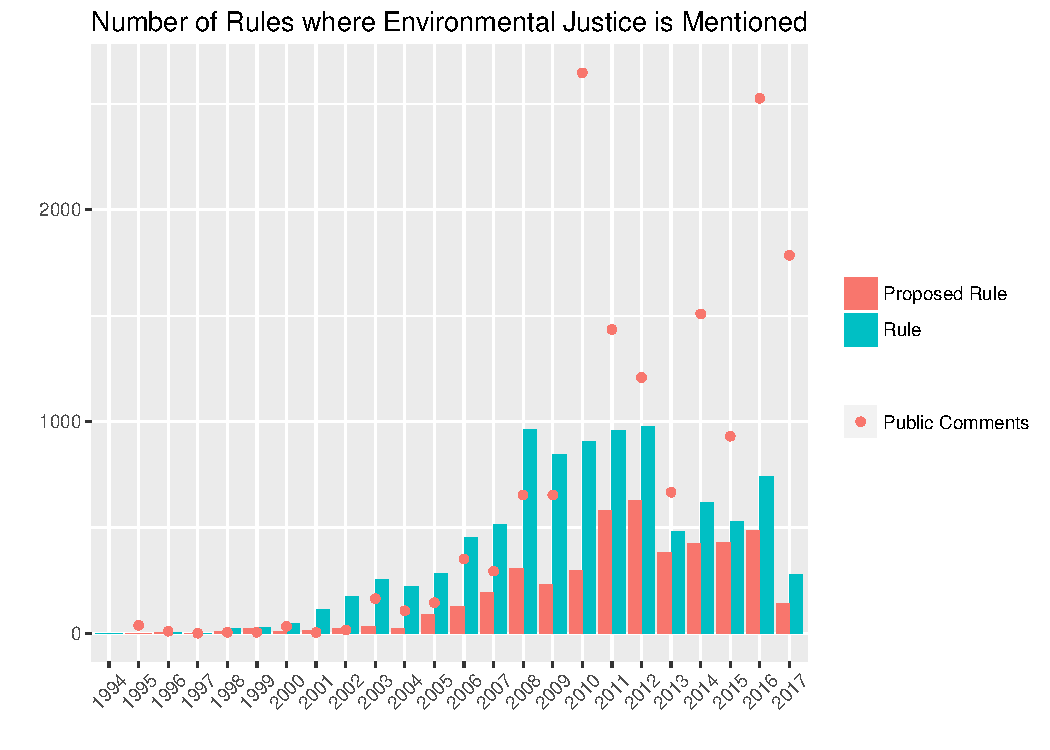
\includegraphics[width = 3.5in]{eandj_hist.pdf}
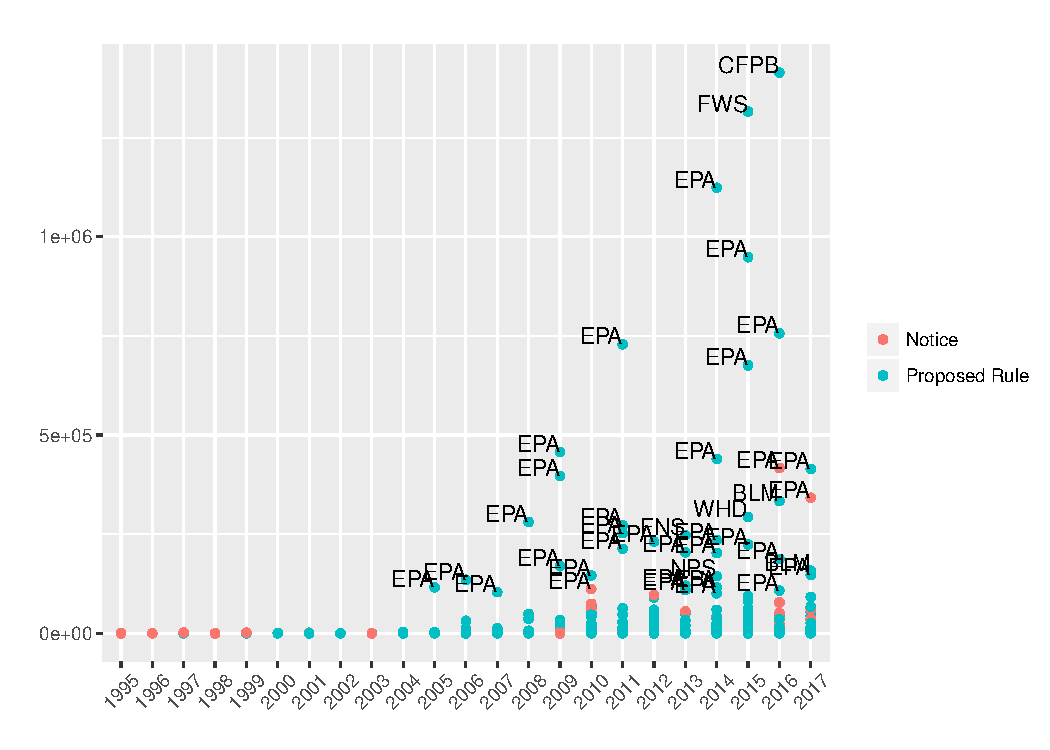
\includegraphics[width =3.5in]{eandj_comments.pdf}
\label{fig:ej}
\end{figure}

Figure \ref{fig:ej} shows that the number of rules and comments increasing over time. This may reflect increased salience of this concept, but it may primarily be the result of the increasing prevalence of searchable texts.  Similarly, the increased number of rules where comments mention environmental justice may reflect growth in the movement but also may reflect more overall comments as technology has made commenting easier. Testing the hypotheses that comments raising environmental justice concerns are related to specific rules where environmental justice is addressed in the final but not in the draft requires rule-specific analysis. 

What we can say from Figure  \ref{fig:ej}  is that each year, more final rules directly address environmental justice when their draft did not. Additionally, there are many rules where environmental justice is mentioned in the public comments and not in the draft. Recently, there are also many rules where environmental justice is raised in the comments but does not make it into the final draft.\footnote{Note that, because not all comments are searchable, this is an underestimate of the number of comments mentioning environmental justice, so we cannot conclude that before 2010, rules were mentioning environmental justice when the comments had not. Additionally, this does not include comments like those of the Bishops who raise justice issues but do not use the phrase ``environmental justice.''} 

% \subsection{Next Steps}
%With these data in hand, the next step is to match each draft and final rule to identify how each changed and to match each comment to its rule to see if the observed changes were suggested in comments. 

\subsubsection{Second-order Representation} Before analysis of whether comments matter, I briefly describe who these commenters are. This is what \citet{Seifter2016Second-OrderLaw} calls ``second-order'' representation. It is insufficient to know which groups participate. We also need to know who these groups represent.

I  investigate who is raising environmental justice concerns in two ways. First, I  identify the top organizational commenters such as tribes, businesses, and nonprofits that are using environmental justice language and investigate who these groups represent. Second, for comments where a citizen signed their name, I  compare surnames to their racial and ethnic identity propensities with respect to the U.S. census. Together these two pieces of information allow me to comment on ``second order'' representation, i.e. not just the extent to which public comments relate to government policy, but the extent to which public comments are representative of the public and of the groups they claim to represent. 


\begin{figure}[!h]
\centering
\begin{tabular}{rlll}
  \hline
 & Organization & Comments & Rules \\ 
  \hline
1 & Earthjustice & 1114782 & 28 \\ 
  2 & Natural Resources Defense Council &  340554 &  8 \\ 
  3 & Sierra Club &  349841 &  5 \\ 
  4 & Alliance for Climate Protection &  253867 &  5 \\ 
  5 & WE ACT for Environmental Justice &    2402 &  3 \\ 
  6 & CREDO &  112879 &  2 \\ 
  7 & Union of Concerned Scientists &   43559 &  2 \\ 
  8 & Earthworks &     308 &  2 \\ 
  9 & Communities for a Better Environment &      21 &  2 \\ 
  10 & Southern Company &       8 &  2 \\ 
  11 & Move On &  165948 &  1 \\ 
  12 & Care2 &   70450 &  1 \\ 
  13 & The Pew Charitable Trusts &   63769 &  1 \\ 
  14 & Hudson-Environmental Action &   35000 &  1 \\ 
  15 & Democracy for America &    4426 &  1 \\ 
  \end{tabular}
  \label{fig:orgs}
  \end{figure}

Figure \ref{fig:orgs} shows the top 15 organizational commenters who used the phrase ``environmental justice'' in their comments, including all organizations who did so on more than one rule or mobilized more than 100,000 such comments. The six organizations responsible for mobilizing more than 100,000 comments and several others on the list are national nonprofit advocacy groups.  We Act and Communities for a Better Environment are both more community-based groups focusing primarily on environmental justice issues. Southern Company is the only corporation on the list
 
 The top mobilizer, Earthjustice, is primarily engaged in litigation on behalf environmental causes. Their website boasts 2.2 million supporters,  but it is not clear who they are or if they play any role in the advocacy strategy. A search on the website returns 360 results for "Environmental Justice," with the top results from staff biographies who work on more local or targeted work such as environmental conditions for the incarcerated, but the environmental justice language used on the main page is relatively mild. For example, ``We are fighting for a future where children can breathe clean air, no matter where they live'' \citep{Earthjustice2017OurWork}. The website does contain Spanish language content. 
 
 The Natural Resources Defense Council is similar to Earthjustice--a national nonprofit funded by donations and focused on litigation--but they also lobby. CREDO Action and MoveOn are more generic progressive mobilizers who lack a systematic focus on environmental justice issues, but occasionally leverage their very large membership lists to support campaigns environmental justice campaigns led by others \citep{MoveOn.org2017MoveOn.OrgAction,CREDO2017CREDOTogether}. The Alliance for Climate Protection is a more of an elite political group founded by former Vice President Al Gore. 
 
 We Act and Communities for a Better Environment both have environmental justice in their central mission statement. We Act was founded by community leaders in Harlem, NY, to fight environmental racisms and advocate for better air quality \citep{WEACT2017WEChange}. Communities for a Better Environment has projects throughout California, but seems particularly active in Oakland \citep{CBECAL2017CommunitiesEnvironment}. Much of the content of their website is in both English and Spanish. Both organizations focus primarily on ``low-income communities of color'' and thus frame their work with respect to race and class. While both organizations participated in national policymaking We Act is more focused on communities in Harlem and New York whereas Communities for a Better Environment casts a wider frame: "CBE’s vision of environmental justice is global--that’s why the organization continues to participate in such international efforts as the Indigenous Environmental Network and the Global Week of Action for Climate Justice" \citep{CBECAL2017CommunitiesEnvironment}.
 
 The Southern Company comments are too few to count as mass mobilization. Companies do sometimes fund mobilization campaigns, but all of 8 of these comments were submitted by the Southern Company. Interestingly, the company repeatedly raises research into environmental justice concerns in order to frame these issues as a legitimate but unresolved scientific debate that is not yet conclusive enough to base regulations on: "People with lower SES are exposed to almost an order of magnitude more traffic near their homes (Reynolds et al., 2001), and live closer to large industrial sites and are exposed to more industrial air pollution (Jerrett et al., 2001). Legitimate health concerns must be addressed. But adopting standards with a scientific basis so uncertain that health improvement cannot be assured is not sound public health policy." Like many companies they claim to represent their customers as "electric generating companies and their customers are expected to bear much of the burden" of regulations \citep{Hobson2004CommentCompany}.
 
 With respect to second-order representation, it appears that the groups most often using the language of environmental justice may do so sincerely, but do not themselves represent affected communities. Several groups representing local communities and led by community leaders have participated, but not nearly as often or with the same intensity as the ``big greens.'' Finally, a third class of commenter appears to be raising environmental justice issues as a way to re-frame them as ongoing debates and thus undermine their urgency. In a way, the fact that an energy company felt compelled to acknowledge and question environmental justice concerns suggests their importance for policy outcomes.

Next, I attempt to estimate the racial distribution of those who comment using environmental justice language. This can only be done for individuals who commented separately from mobilizing organizations and signed their full name on their comment. 
Figure \ref{ejcommentsbyrace} shows two ways of estimating the racial distribution of commenters who raise ``environmental justice'' concerns in their comments. Both methods use the reported racial identities associated with surnames as recorded in the 2010 census\footnote{I recode ``Hispanic'' as ``Latinx'' in both cases because the prediction method assumes a forced choice that includes ``Hispanic'' as a primary racial category} and are based on a limited sample of 327 commenters who signed their name with a surname matching census records.  The first is based on the proportion of people with a given surname that identified as belonging to each racial category (from this limited set of options). The estimated proportion of each race for this sample is simply the average of proportions identified with each surname. This is likely the most accurate way to represent the racial distribution of a set of surnames, but it does not assign specific individuals to racial categories. The second method does. It predicts the race of each individual in the sample based on their surname given the distribution of racial categories reported by people with that surname and the proportion of each race in the U.S. population. Thus, while a surname may be more common among people who identify as black rather than as white, there may still be more White people with that surname and this method would predict that the person is White. For this reason, the portion of individuals predicted to be White (right) is higher than in the probabilistic distribution (left). 

\begin{figure}[h!]
\caption{Probabilistic (Left) and Predicted (Right) Race from Census Surnames}
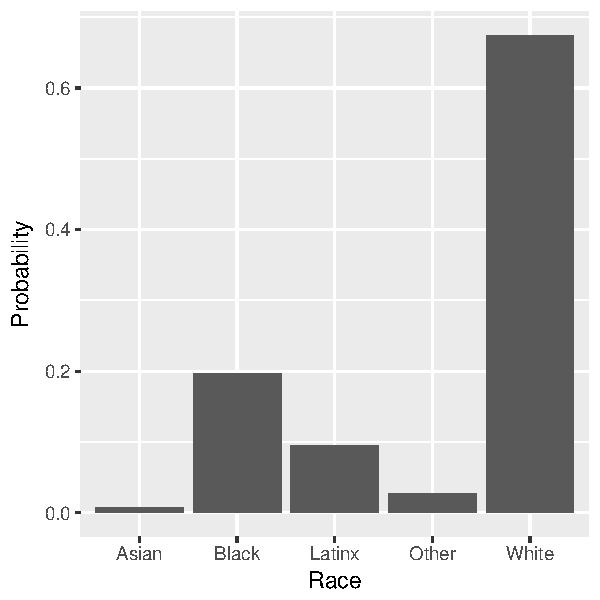
\includegraphics[width = 3in]{race_prob.pdf}
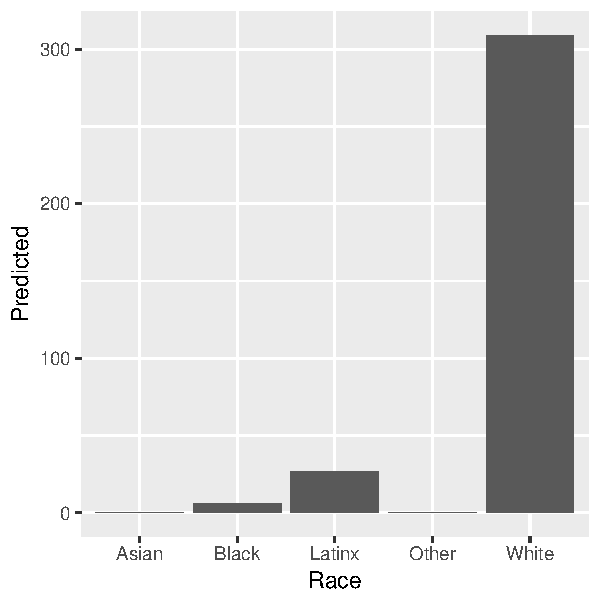
\includegraphics[width = 3in]{race_pred.pdf}
\label{ejcommentsbyrace}

\end{figure}

Compared to estimates from the 2010 census, this sample of commenters is disproportionately Black and less than proportionally Latinx or Asian, with just slightly fewer Whites relative to the national population. 

Figure \ref{ejwordsbyrace} shows the most common words used in comments with respect to the predicted race of each commenter in the sample. As there are very few predicted non-White commenters in the sample, it is unwise to infer too much from this figure. 


\begin{figure}[h!]
\caption{Common Words by Race}
\begin{tabular}{ccc}
White & Latinx & Black\\

\includegraphics[width = 2in]{ej_white_words.pdf}
&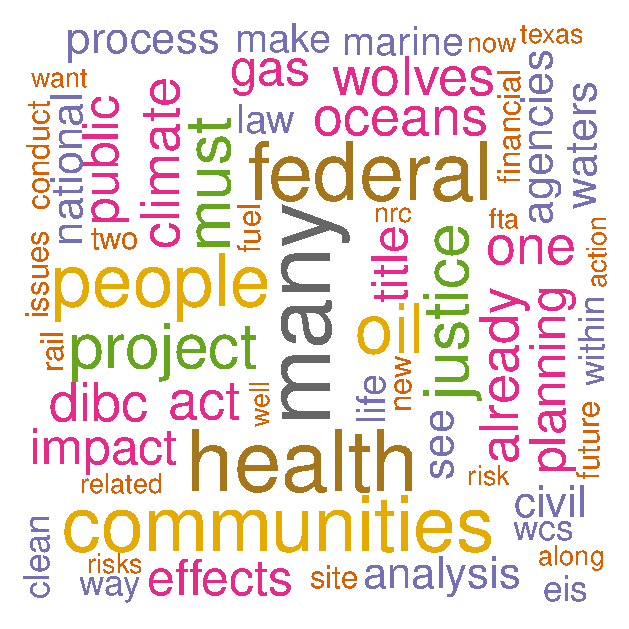
\includegraphics[width = 2in]{ej_latinx_words.pdf}
&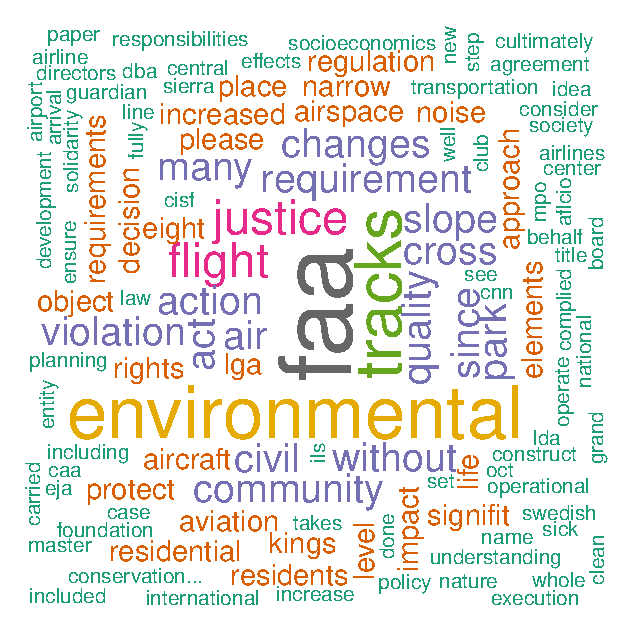
\includegraphics[width = 2in]{ej_black_words.pdf}
\end{tabular}
\label{ejwordsbyrace}
\end{figure}

% Time allowing I will also investigate different pathways to influence such as how rule-specific environmental justice concerns were raised in congressional hearings and reports. 


\subsection{Results: Are final rules more likely to address environmental justice after comments do so?}


This subsection presents results from an analysis of draft rules, comments, and final rules. Descriptively, figure \ref{ejwinrate} shows that in general, most rules that do not address environmental justice in the draft but these issues are raised in the comments, do not end up addressing them in the final version. It appears that it may have been the case in 2006 and 2007 but since then the number of rules receiving comments raising environmental justice concerns has grown while the number of rules that end up adding it has remained the same. Since 2015, there has been a decline in both the number of rules adding environmental justice and the number of rules where commenters demanded it, especially in 2017. One way to interpret figure \ref{ejwinrate} would be to say that commenters saw a potential ally in President Obama and increased their demands for environmental justice, but that these increased demands had little effect. However, a better approach would be to estimate a statistical model of the effect of comments on the change from draft to final rules. This is what I do.


\begin{figure}[h!]
\caption{Rules With Comments Addressing EJ on a Draft That Did Not}
\centering
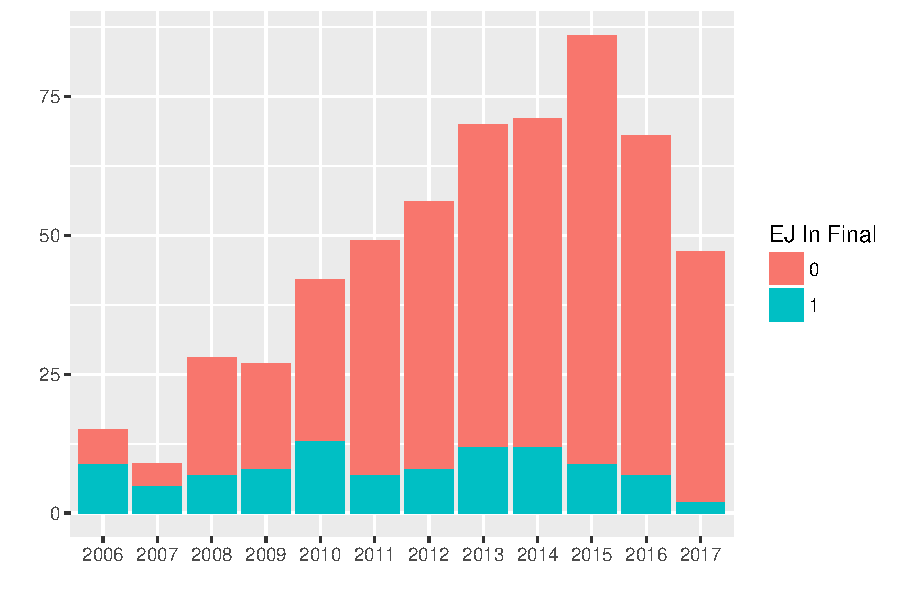
\includegraphics[width = 3.5in]{ej_win_rate.pdf}
\label{ejwinrate}
\end{figure}




I estimate a logit regression where the outcome is whether environmental justice was addressed in the final rule and the predictors are whether it was addressed in the draft rule, whether it was addressed in the comments, and the total number of comments received. 

\begin{align*}
  \hat{EJ in Final} = \Bigg\{ \begin{array}{lll}
    1 & if &  \beta_0 + \beta_1 EJ in Draft + \beta_2 EJ in Comments + \beta_3 Total Comments  + \epsilon > 0\\
0 & otherwise &  
  \end{array}
\end{align*}

As logit coefficients are not easily interpretable, I calculate predicted probabilities for the types of rules of interest, i.e. rules where environmental justice was not raised in the draft, \textit{EJinDraft}=0.  Figure \ref{ejpredicted} shows the predicted probability of a final rule addressing environmental justice when the draft rule did not for all agencies that have ever published a rule addressing environmental justice (left) and the EPA alone (right). The EPA accounts for nearly two-thirds of the cases where environmental justice is raised in the comments on a draft rule that did not address it. We see that the total number of comments has no effect. In contrast, environmental justice being raised in the comments has a statistically significant and substantively large effect. 

Overall the probability across all agencies of adding environmental justice increases from under 2\% to about 9\%. At the EPA, the probability triples from about 6\% to about 18\%. 


\begin{figure}[h!]
\caption{Proposed Rules Not Addressing Environmental Justice (Left: All agencies. Right: Environmental Protection Agency)}
\centering
\noindent
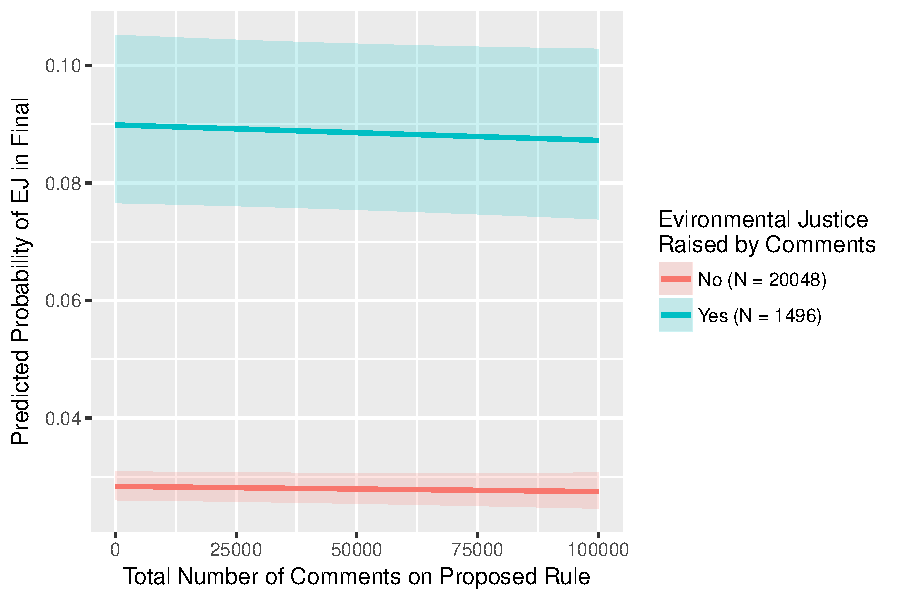
\includegraphics[width = 3.2 in]{ej_prob_env_nprms.pdf}
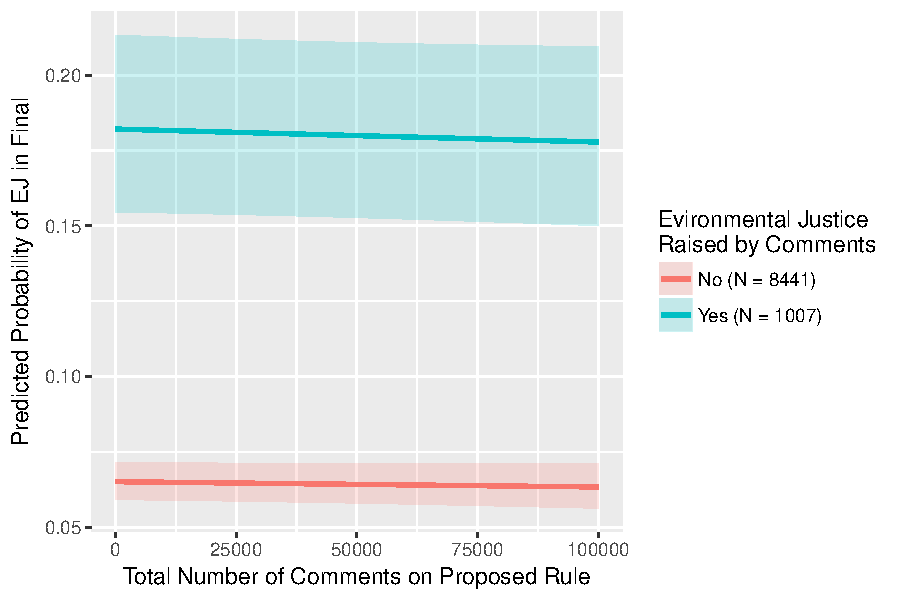
\includegraphics[width = 3.2 in]{ej_prob_epa_nprms.pdf}
\label{ejpredicted}
\end{figure}

To examine the degree to which this result is generalizable, figure \ref{ejlogitagencies} presents predicted probabilities for each agency, showing that the range of predicted probabilities are systematically higher when environmental justice. There is considerable variation among agencies and only a few agencies have statistically significant different estimates, but the agencies where effects are largest and most significant are exactly the agencies we would expect to be influenced by comments raising environmental justice concerns. They are agencies that deal with environmental issues with distributive consequences. 


\begin{figure}[h!]
\caption{Proposed Rules Not Addressing Environmental Justice}
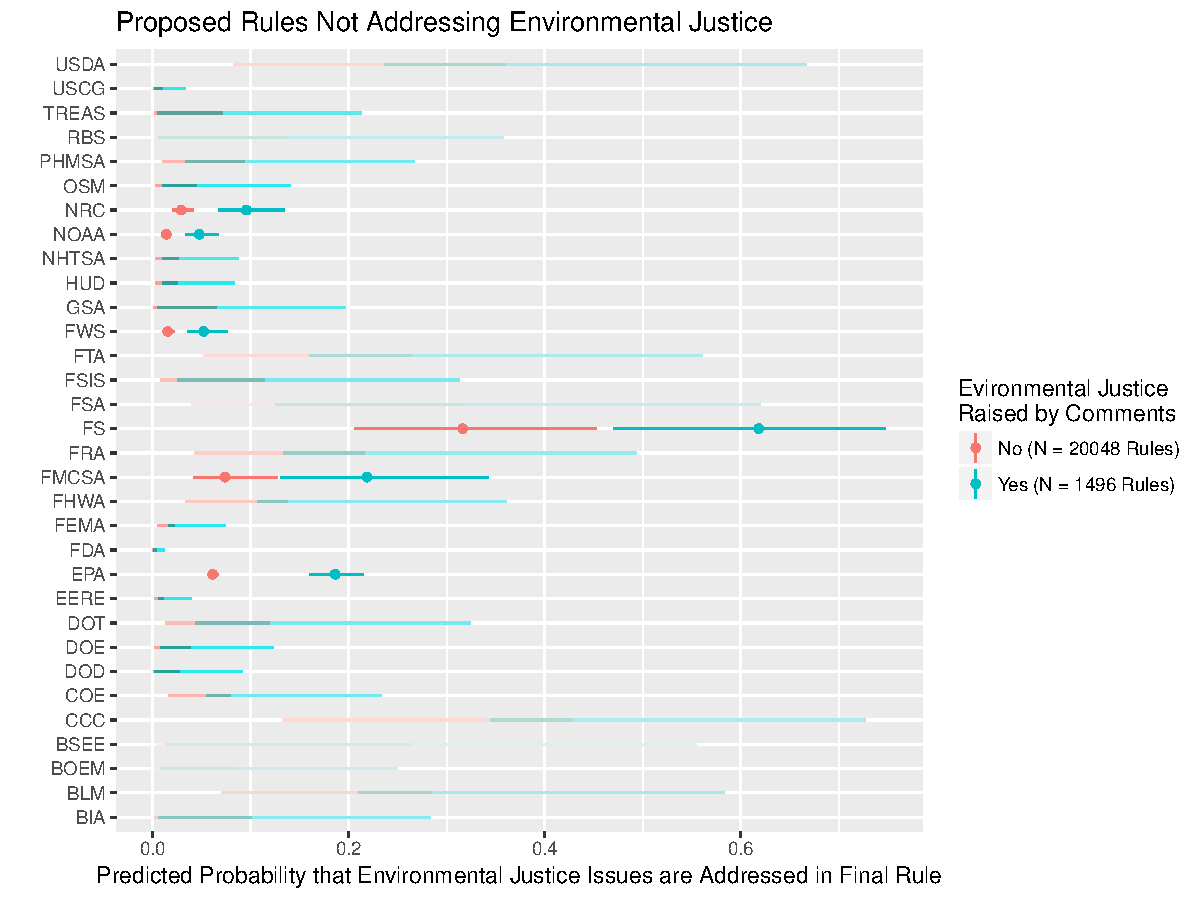
\includegraphics[width = \textwidth]{ej_prprob_by_agency.pdf}
\label{ejlogitagencies}

\end{figure}

As the EPA accounts for the largest portion of the data, we are most confident in this result, but the EPA is not the agency with the largest predicted effects. The Forest Service has a predicted 30\% difference between rules that do and do not receive comments raising environmental justices concerns. This may be because the forest service is mainly in the business of managing forests, leasing timber rights, and controlling wildfires. These types of decisions may have acute distributional effects that may not be the initial focus of the agency. Once raised, however, addressing such effects fits squarely in their mission. Though not statically significant the Department of Agriculture and Bureau of Land Management, who make similar kinds of decisions, also have large predicted probabilities. Similarly, the Federal Railroad Administration, Department of Transportation, Federal Highway Administration, Federal Motor Carrier Safety Administration, and Federal Transportation Administration (which aids local transportation projects) all have large probability distributions. These agencies are making decisions about infrastructure projects with implications for neighborhood environments and air quality. Environmental justice may often come up, but there may be a lot of variation in whether the agency then decides if they are relevant to transportation policies and projects that are primarily about neither environmental nor justice concerns. 

Research agencies, including the National Research Council, National Oceanographic and Atmospheric Administration and Fish and Wildlife Service all had statistically significant but small spreads. In these cases, we can be confident of the correlation, but understand that it is a rare occurrence, which makes sense if most research does not have direct environmental justice consequences, but agencies are open to adding analysis of these issues if when they are raised. 

\section{Conclusion}
This analysis has illustrated the importance of ideas in policymaking and cross-sectional statistical results suggest that rules where issue frame like environmental justice are raised have a higher probability that policymakers consider the effects on marginalized populations. Importantly this relationship seems to be conditional on an institutional environment that is predisposed to such an analysis. Furthermore, it is important to note that the policy outcomes suggested by environmental justice analysis depend on how minority populations are defined. In some cases, those raising environmental justice concerns present it as an issue of wealth or income inequality, leading policy to account for disparate impacts on low-income populations. In other cases, groups raise claims rooted in cultural practices, such as fish consumption among certain tribes. As occurred in the Mercury Rule, analysis in subsequent drafts of the policy used evaluative criteria specific to these communities. 

The ability of a frame like environmental justice to construct certain populations as deserving of consideration means that policy outcomes will depend on the specific environmental justice concerns raised. In this respect, second-order representation may become important. National  advocacy organizations may frequently request that regulators protect ``all people'' or even ``low-income communities of color.'' However, this more generic advocacy may not lead to the same outcomes as groups that present specific local environmental justice grievances that are unique to a community. In between generic progressive advocacy organizations and community-based organizations are organizations like Earthjustice who, despite their national focus, frequently engaged in community-specific litigation and thus raise these local concerns in national policymaking. 

In the end, the above analysis offers some clarity on a poorly understood but important mechanism of American policymaking. It offers some hope that citizen opinions may be heard through direct democracy institutions built into bureaucratic policymaking.  The examination of second-order participation validates some of the skepticism about who participates. It is elite groups who participate, even with respect to an issue like environmental justice. However, government responsiveness does not seem to depend on mass mobilization or elite support. Compared to cases where environmental justice issues were not raised, when they are, we see a significantly higher probability that they will be addressed by policymakers. 

% Chapter 7 Field Experiments / Contemporary Case Studies

% Chapter 8 Conclusion

% Appendix 
% Survey



% \theendnotes
\singlespace
\small
\bibliographystyle{apsr.bst} 
\bibliography{Mendeley.bib}
\end{document}





